% Dokumentenkopf ---------------------------------------------------------------
%   Diese Vorlage basiert auf "scrreprt" aus dem koma-script.
% ------------------------------------------------------------------------------

\documentclass[
    11pt, % Schriftgr��e
    DIV10,
    ngerman, % f�r Umlaute, Silbentrennung etc.
    a4paper, % Papierformat
    open=right,
    oneside, % einseitiges Dokument
    titlepage, % es wird eine Titelseite verwendet
    parskip=half*, % Abstand zwischen Abs�tzen (halbe Zeile)
    headings=normal, % Gr��e der �berschriften verkleinern
    listof=totoc, % Verzeichnisse im Inhaltsverzeichnis auff�hren
    bibliography=totoc, % Literaturverzeichnis im Inhaltsverzeichnis auff�hren
    index=totoc, % Index im Inhaltsverzeichnis auff�hren
    captions=tableheading, % Beschriftung von Tabellen unterhalb ausgeben
    final % Status des Dokuments (final/draft)
]{scrreprt}
%\setlength{\parskip}{0pt}
\newtheorem{bsp}{Beispiel}[chapter]
% Meta-Informationen -----------------------------------------------------------
%   Informationen �ber das Dokument, wie z.B. Titel, Autor, Matrikelnr. etc
%   werden in der Datei Meta.tex definiert und k�nnen danach global
%   verwendet werden.
% ------------------------------------------------------------------------------
% Meta-Informationen -----------------------------------------------------------
%   Definition von globalen Parametern, die im gesamten Dokument verwendet
%   werden k�nnen (z.B auf dem Deckblatt etc.).
%
%   ACHTUNG: Wenn die Texte Umlaute oder ein Esszet enthalten, muss der folgende
%            Befehl bereits an dieser Stelle aktiviert werden:
            \usepackage[latin1]{inputenc}
% ------------------------------------------------------------------------------
\newcommand{\titel}{Support Vector Machines}
\newcommand{\untertitel}{}
\newcommand{\art}{Seminar}
\newcommand{\arttitel}{--Regularisierungstechniken und strukturierte Regression--}
%\newcommand{\fachgebiet}{Software-Engineering}
\newcommand{\autor}{Giuseppe Casalicchio}
%\newcommand{\studienbereich}{Software-Engineering}
\newcommand{\matrikelnr}{8049501}
\newcommand{\erstgutachter}{Prof. Dr. Gerhard Tutz}
\newcommand{\zweitgutachter}{Wolfgang P��necker}
\newcommand{\jahr}{8. M�rz 2013}
\newcommand{\efp}{\text{\textit{efp}}}
%\newcommand{\ort}{Berlin}
%\newcommand{\logo}{lmu_siegel.pdf}




%%\usepackage[utf8]{inputenc}
%\usepackage{german}

%%% Zaehler fuer Aufgaben
\newcounter{ex}
\setcounter{ex}{0}
\newcommand{\ex}{\item{\stepcounter{ex} \textbf{Aufgabe
                       \arabic{ex} }}\newline}


%%% Theoremumgebungen
\usepackage{amsmath}
\usepackage{amssymb}
\usepackage{amsthm}

   \newtheoremstyle{ththm}% name
     {\topsep}%      Space above
     {\topsep}%      Space below
     {\normalfont}%         Body font
     {}%         Indent amount (empty = no indent, \parindent = para indent)
     {\normalfont\bfseries}% Thm head font
     {}%        Punctuation after thm head
     {\newline}%     Space after thm head: " " = normal interword space;
           %       \newline = linebreak
     {\thmname{#1}\thmnumber{ #2}\thmnote{ (#3)}}%         Thm head spec (can be left empty, meaning `normal')



%% Definition
\theoremstyle{ththm}
\newtheorem{defi}{Definition}[chapter]
\newtheorem{satz}[defi]{Satz}
\newtheorem{lemma}[defi]{Lemma}
\newtheorem{korollar}[defi]{Korollar}
\newtheorem{beispiel}{Beispiel}[chapter]

\theoremstyle{remark}
\newtheorem*{beme}{Bemerkung}

\newenvironment{beweis}{\begin{proof}[Beweis] \textcolor{white}{weiss} \newline}{\end{proof}}


% ben�tigte Packages -----------------------------------------------------------
%   LaTeX-Packages, die ben�tigt werden, sind in die Datei Packages.tex
%   "ausgelagert", um diese Vorlage m�glichst �bersichtlich zu halten.
% ------------------------------------------------------------------------------
% Anpassung des Seitenlayouts --------------------------------------------------
%   siehe Seitenstil.tex
% ------------------------------------------------------------------------------
\usepackage[
    automark, % Kapitelangaben in Kopfzeile automatisch erstellen
    headsepline, % Trennlinie unter Kopfzeile
    ilines % Trennlinie linksb�ndig ausrichten
]{scrpage2}

% Sweave --------------------------------------------------------------------
\usepackage{Sweave}
%\usepackage{enumitem}
%\usepackage{textcomp}

%\SweaveOpts{eps=FALSE,keep.source=FALSE}

% Anpassung an Landessprache ---------------------------------------------------
\usepackage[ngerman]{babel}

% Umlaute ----------------------------------------------------------------------
%   Umlaute/Sonderzeichen wie ���� direkt im Quelltext verwenden (CodePage).
%   Erlaubt automatische Trennung von Worten mit Umlauten.
% ------------------------------------------------------------------------------
\usepackage[latin1]{inputenc}

\usepackage[T1]{fontenc}
\usepackage{textcomp} % Euro-Zeichen etc.

% Schrift ----------------------------------------------------------------------
\usepackage{lmodern} % bessere Fonts
\usepackage{relsize} % Schriftgr��e relativ festlegen

% Grafiken ---------------------------------------------------------------------
% Einbinden von JPG-Grafiken erm�glichen
%\usepackage[dvips,final]{graphicx}
% hier liegen die Bilder des Dokuments
\graphicspath{{Bilder/}}

% Befehle aus AMSTeX f�r mathematische Symbole z.B. \boldsymbol \mathbb --------
\usepackage{amsthm,amsmath,amsfonts}

% f�r Index-Ausgabe mit \printindex --------------------------------------------
%\usepackage{makeidx}

% Einfache Definition der Zeilenabst�nde und Seitenr�nder etc. -----------------
\usepackage{setspace}
\usepackage{geometry}

% Symbolverzeichnis ------------------------------------------------------------
%   Symbolverzeichnisse bequem erstellen. Beruht auf MakeIndex:
%     makeindex.exe %Name%.nlo -s nomencl.ist -o %Name%.nls
%   erzeugt dann das Verzeichnis. Dieser Befehl kann z.B. im TeXnicCenter
%   als Postprozessor eingetragen werden, damit er nicht st�ndig manuell
%   ausgef�hrt werden muss.
%   Die Definitionen sind ausgegliedert in die Datei "Glossar.tex".
% ------------------------------------------------------------------------------
%\usepackage[intoc]{nomencl}
%\let\abbrev\nomenclature
%\renewcommand{\nomname}{Abk�rzungsverzeichnis}
%\setlength{\nomlabelwidth}{.25\hsize}
%\renewcommand{\nomlabel}[1]{#1 \dotfill}
%\setlength{\nomitemsep}{-\parsep}

% zum Umflie�en von Bildern ----------------------------------------------------
\usepackage{floatflt}


% zum Einbinden von Programmcode -----------------------------------------------
\usepackage{listings}
\usepackage{xcolor} 
%\definecolor{hellgelb}{rgb}{1,1,0.9}
\definecolor{hellgelb}{rgb}{1,1,1}
\definecolor{colKeys}{rgb}{0,0,0} %0,0,1
\definecolor{colIdentifier}{rgb}{0,0,0}
\definecolor{colComments}{rgb}{0,0,0} %1,0,0
\definecolor{colString}{rgb}{0,0,0} %0,0.5,0
\lstset{
    language=R, 
    float=hbp,
    basicstyle=\ttfamily\color{black}\small,
    identifierstyle=\color{colIdentifier},
    keywordstyle=\color{colKeys},
    stringstyle=\color{colString},
    commentstyle=\color{colComments},
    columns=flexible,
    tabsize=2,
    frame=single,
    extendedchars=true,
    showspaces=false,
    showstringspaces=false,
    numbers=left,
    numberstyle=\tiny,
    breaklines=true,
    backgroundcolor=\color{hellgelb},
    breakautoindent=true
}

% URL verlinken, lange URLs umbrechen etc. -------------------------------------
\usepackage{url}

% wichtig f�r korrekte Zitierweise ---------------------------------------------
\usepackage[round]{natbib}

% PDF-Optionen -----------------------------------------------------------------
\usepackage[
    bookmarks,
    bookmarksopen=true,
    %%%%%%%%%%%%%%%%%%%%%%%%%%%%%%%%%%%%%
    colorlinks=true, % diese Farbdefinitionen zeichnen Links im PDF farblich aus
    linkcolor=red, % einfache interne Verkn�pfungen
    anchorcolor=black,% Ankertext
    citecolor=blue, % Verweise auf Literaturverzeichniseintr�ge im Text
    filecolor=magenta, % Verkn�pfungen, die lokale Dateien �ffnen
    menucolor=red, % Acrobat-Men�punkte
    urlcolor=cyan,     
%	backref, % R�ckverweis aus Literaturverzeichnis
	%%%%%%%%%%%%%%%%%%%%%%%%%%%%%%%%%%%%%%%
%% diese Farbdefinitionen sollten f�r den Druck verwendet werden (alles schwarz)
% 	colorlinks=true,
%     linkcolor=black, % einfache interne Verkn�pfungen
%     anchorcolor=black, % Ankertext
%     citecolor=black, % Verweise auf Literaturverzeichniseintr�ge im Text
%     filecolor=black, % Verkn�pfungen, die lokale Dateien �ffnen
%     menucolor=black, % Acrobat-Men�punkte
%     urlcolor=black, 
	%%%%%%%%%%%%%%%%%%%%%%%%%%%%%%%%%%%%%%
    plainpages=false, % zur korrekten Erstellung der Bookmarks
    pdfpagelabels, % zur korrekten Erstellung der Bookmarks
    hypertexnames=false, % zur korrekten Erstellung der Bookmarks
    linktocpage % Seitenzahlen anstatt Text im Inhaltsverzeichnis verlinken
]{hyperref}
% Befehle, die Umlaute ausgeben, f�hren zu Fehlern, wenn sie hyperref als Optionen �bergeben werden
\hypersetup{
    pdftitle={\titel \untertitel},
    pdfauthor={\autor},
    pdfcreator={\autor},
    pdfsubject={\titel \untertitel},
    pdfkeywords={\titel \untertitel},
}

% fortlaufendes Durchnummerieren der Fu�noten ----------------------------------
\usepackage{chngcntr}

% f�r lange Tabellen ----------------------------------------------------------
\usepackage{longtable}
\usepackage{array}
\usepackage{ragged2e}
\usepackage{lscape}

% Spaltendefinition rechtsb�ndig mit definierter Breite ------------------------
\newcolumntype{w}[1]{>{\raggedleft\hspace{0pt}}p{#1}}

% Formatierung von Listen �ndern -----------------------------------------------
\usepackage{paralist}

% bei der Definition eigener Befehle ben�tigt
\usepackage{ifthen}

% definiert u.a. die Befehle \todo und \listoftodos
\usepackage{todonotes}

% sorgt daf�r, dass Leerzeichen hinter parameterlosen Makros nicht als Makroendezeichen interpretiert werden
\usepackage{xspace}

\usepackage{framed, color}
\usepackage{multicol}
\usepackage{cancel}



% Erstellung eines Index und Abk�rzungsverzeichnisses aktivieren ---------------
%\makeindex
%\makenomenclature

% Kopf- und Fu�zeilen, Seitenr�nder etc. ---------------------------------------
% Zeilenabstand 1,5 Zeilen -----------------------------------------------------
\onehalfspacing

% Seitenr�nder -----------------------------------------------------------------
\setlength{\topskip}{\ht\strutbox} % behebt Warnung von geometry
\geometry{paper=a4paper,left=30mm,right=30mm,top=30mm}

% Kopf- und Fu�zeilen ----------------------------------------------------------
\pagestyle{scrheadings}
% Kopf- und Fu�zeile auch auf Kapitelanfangsseiten
\renewcommand*{\chapterpagestyle}{scrheadings} 
% Schriftform der Kopfzeile
\renewcommand{\headfont}{\normalfont}

% Kopfzeile alt mit fehler
%\ihead{
%%\large{\textsc{\titel}}\\ \small{\untertitel} \\[2ex] 
%\textit{\headmark}}
%\chead{}
%%\ohead{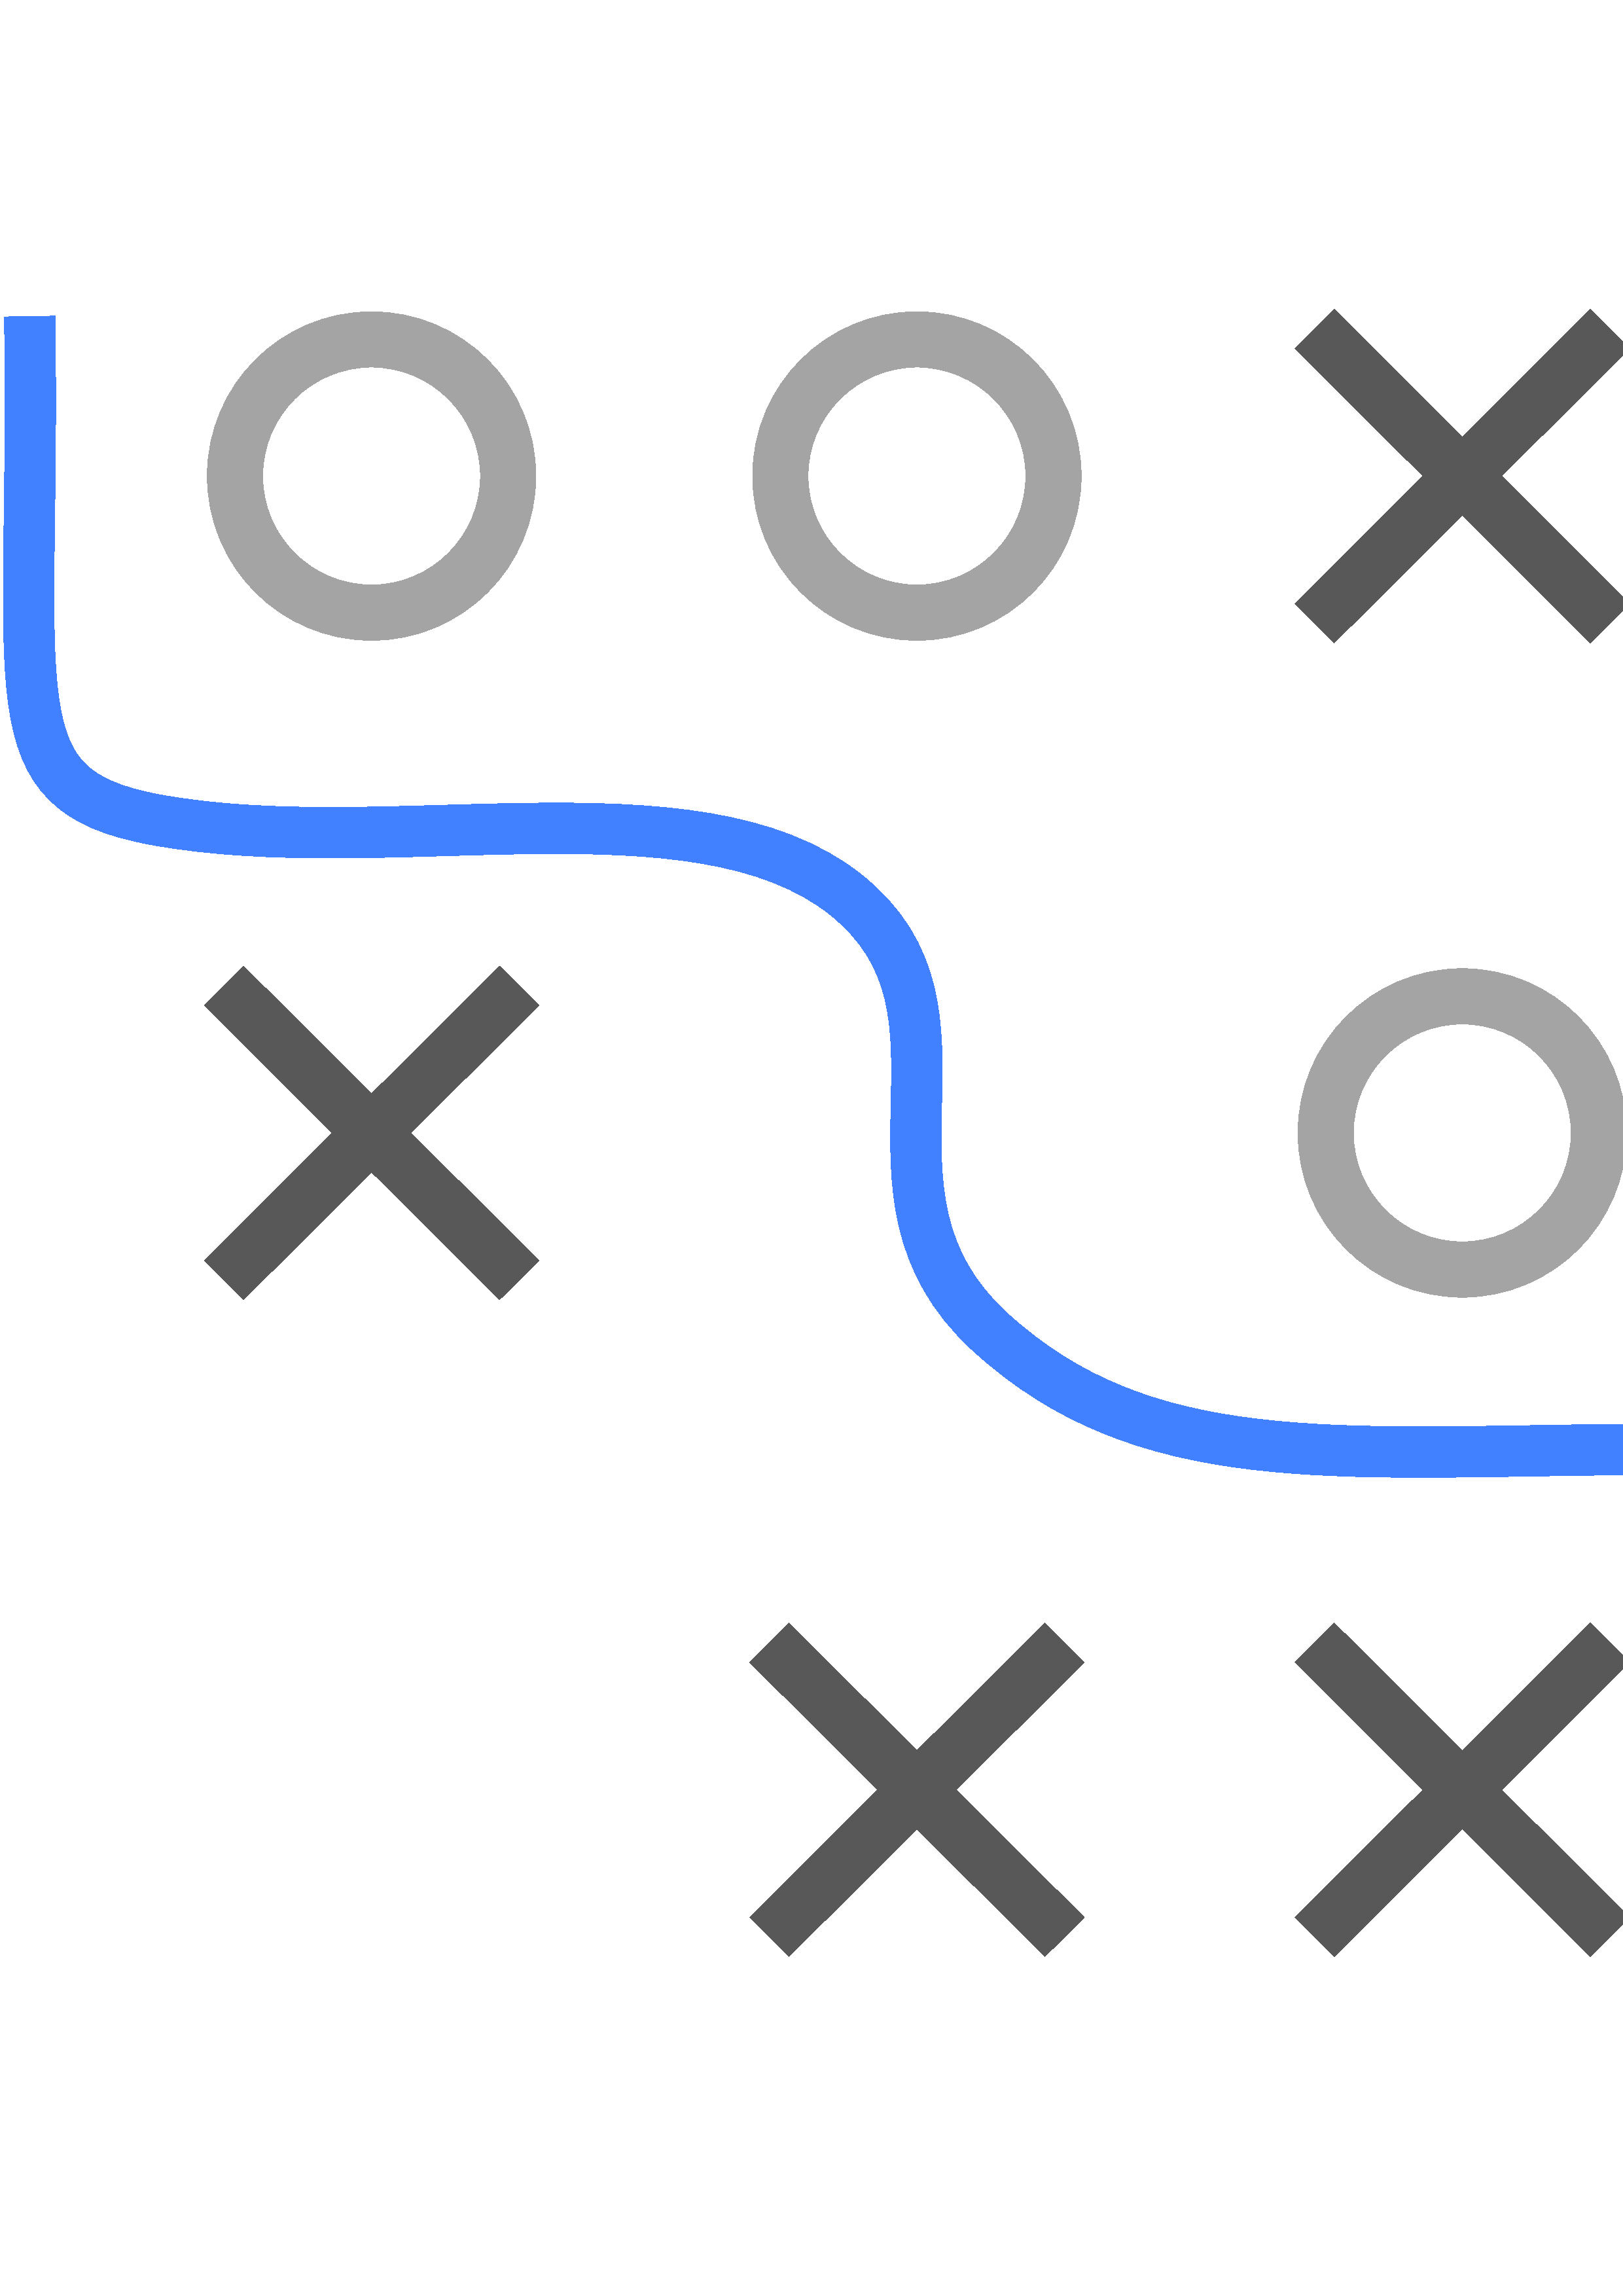
\includegraphics[scale=0.15]{\logo}}
%\setlength{\headheight}{21mm} % H�he der Kopfzeile
%% Kopfzeile �ber den Text hinaus verbreitern
%\setheadwidth[0pt]{textwithmarginpar} 
%\setheadsepline[text]{0.4pt} % Trennlinie unter Kopfzeile


% Kopfzeile
%\ihead{\textit{\headmark}}
%\chead{}
%\setlength{\headheight}{21mm} % H�he der Kopfzeile
% Kopfzeile �ber den Text hinaus verbreitern
%\setheadwidth[0pt]{textwithmarginpar} 
%\setheadsepline[text]{0.4pt} % Trennlinie unter Kopfzeile



% Fu�zeile
%\ifoot{\copyright\ \autor}
%\cfoot{}
%\ofoot{\pagemark}

% sonstige typographische Einstellungen ----------------------------------------

% erzeugt ein wenig mehr Platz hinter einem Punkt
\frenchspacing 

% Schusterjungen und Hurenkinder vermeiden
\clubpenalty = 10000
\widowpenalty = 10000 
\displaywidowpenalty = 10000

% Quellcode-Ausgabe formatieren
\lstset{numbers=left, numberstyle=\tiny, numbersep=5pt, breaklines=true}
\lstset{emph={square}, emphstyle=\color{red}, emph={[2]root,base}, emphstyle={[2]\color{blue}}}

% Fu�noten fortlaufend durchnummerieren
%\counterwithout{footnote}{chapter}


\newcommand{\sgn}{\operatorname{sgn}}
% Das eigentliche Dokument -----------------------------------------------------
%   Der eigentliche Inhalt des Dokuments beginnt hier. Die einzelnen Seiten
%   und Kapitel werden in eigene Dateien ausgelagert und hier nur inkludiert.
% ------------------------------------------------------------------------------

\allowdisplaybreaks[1]
\begin{document}

% auch subsubsection nummerieren
\setcounter{secnumdepth}{3}
\setcounter{tocdepth}{3}

% Deckblatt und Abstract ohne Seitenzahl
%\ofoot{}
\thispagestyle{empty}
\cleardoublepage
\thispagestyle{plain}
\begin{titlepage}

\begin{center}
{\Huge INSTITUT F�R STATISTIK\\[1mm]}
DER LUDWIG--MAXIMILIANS--UNIVERSIT�T M�NCHEN\\
\vspace*{1cm}


\includegraphics[width=0.3\textwidth]{lmu_siegel}\\[6ex]

\LARGE{\textbf{\art}}\\[1.5ex]
\Large{\textbf{\arttitel}}\\%[18ex]

\vspace*{\fill}
\huge{\textbf{\titel}}\\[1.5ex]
\LARGE{\textbf{\untertitel}}\\[6ex]
\vspace*{\fill}

\normalsize
\begin{tabular}{ll}\\
Autor:  & \quad \autor\\[1.2ex]
%Studienbereich: & \quad \studienbereich\\[1.2ex]
%Matrikelnummer: & \quad \matrikelnr\\[1.2ex]
%Gutachter:  & \quad \erstgutachter\\[1.2ex]
Betreuer: & \quad \zweitgutachter\\[1.2ex]
Abgabe: & \quad \jahr\\[1.2ex]
%Zweitgutachter: & \quad \zweitgutachter\\[3ex]
\end{tabular}

%\copyright\ \jahr\\[9ex]
\end{center}

\singlespacing
\small

\end{titlepage}


%\thispagestyle{empty}
%\cleardoublepage
%\vspace*{2cm}

\begin{center}
    \textbf{Abstract}
\end{center}

\vspace*{1cm}

\noindent Die vorliegende Bachelorarbeit befasst sich mit dem Testen auf Strukturbr�che unter Verwendung eines generalisierten M-Fluktuationsprozesses, der zur Erfassung von Schwankungen in einem Modell verwendet werden kann. Falls Strukturbr�che vorhanden sind, wird eine Methode vorgestellt, die das Lokalisieren von Strukturbr�chen erm�glicht. Dar�ber hinaus wird das Konzept des Monitorings kurz erl�utert, welches mit Hilfe eines historischen Datensatzes bei neu hinzukommenden Beobachtungen strukturelle Ver�nderungen aufdecken kann. Diese Methoden werden anhand von Daten der An- und Abfl�ge des Flughafen M�nchen illustriert.
%Falls Strukturbr�che in einem Modell vorhanden sind, wird eine Methode vorgestellt. 



\thispagestyle{empty}
\cleardoublepage

%\ofoot{\pagemark}

% Seitennummerierung -----------------------------------------------------------
%   Vor dem Hauptteil werden die Seiten in gro�en r�mischen Ziffern 
%   nummeriert.
% ------------------------------------------------------------------------------
\pagenumbering{roman}
\tableofcontents % Inhaltsverzeichnis
%\listoffigures % Abbildungsverzeichnis

% Abk�rzungsverzeichnis --------------------------------------------------------
%\input{Inhalt/Glossar}
% f�r korrekte �berschrift in der Kopfzeile
%\clearpage\markboth{\nomname}{\nomname} 
%\printnomenclature
%\label{sec:Glossar}

%\listoftables % Tabellenverzeichnis ---------------------------------------------
%\renewcommand{\lstlistlistingname}{Verzeichnis der Listings}
%\lstlistoflistings % Listings-Verzeichnis

% arabische Seitenzahlen im Hauptteil ------------------------------------------
\clearpage
\pagenumbering{arabic}

% die Inhaltskapitel -------------------------

\chapter{Grundlagen}
\label{grundlagen}

%\section{Lagrange-Methode}
%\section{Datensituation
%\textbf{Ausgangslage}:

Bei der Klassifizierung durch Support Vector Machines geht man von $N$ Trainingsdaten $(\mathbf{x}_1^{\top}, y_1), \hdots, (\mathbf{x}_N^{\top}, y_N)$ aus, wobei

\begin{tabular}{lll}
&$\mathbf{x}_i^{\top} \in \mathbb{R}^p$ & ein Merkmalsvektor mit $p$ Variablen und\\
&$y_i \in \{-1,+1\}$ & die Klassenzugeh�rigkeit der $i$-ten Beobachtung
\end{tabular}

ist. Die vorliegende Seminararbeit beschr�nkt sich auf die bin�re Klassifizierung durch Support Vector Machines. Die grundlegende Idee besteht darin, die Daten durch eine Hyperebene in zwei Klassen aufzuteilen. Eine Hyperebene trennt dabei einen $p$-dimensionalen Variablenraum in zwei Halbr�ume und hat selbst die Dimension $(p-1)$. Die Gleichung einer Hyperebene hat die Form
\begin{equation} 
\label{hyperebene}
%\mathcal{H} = 
\{\mathbf{x} \in \mathbb{R}^p \; | \; \mathbf{w}^\top \mathbf{x}+ b = 0\}, 
\end{equation}
wobei $\mathbf{w} \in \mathbb{R}^p$ ein Vektor orthogonal zur Hyperebene und $b \in \mathbb{R}$ die Verschiebung (vom Ursprung) ist.
Beispielsweise sind Hyperebenen
\begin{itemize}
\item in einem eindimensionalen Variablenraum alle Mengen, die aus einem Punkt bestehen,
\item in einem zweidimensionalen Variablenraum alle Geraden und
\item in einem dreidimensionalen Variablenraum alle Ebenen.
\end{itemize}

% Im eindimensionalen Variablenraum ($p=1$) ist jede Mengen, die aus einem Punkt besteht eine Hyperebene.

Das Ziel ist hierbei mit Hilfe einer Entscheidungsfunktion $f: \mathbb{R}^p \rightarrow \{-1,+1\}$ neu hinzukommende Beobachtungen $\mathbf{x}_{neu}$ m�glichst fehlerfrei in die negative Klasse $y_{neu}=-1$ oder in die positive Klasse $y_{neu}=+1$ zuzuordnen. Die Entscheidungsfunktion wird auf Basis der Trainingsdaten so bestimmt, dass der Ausdruck $f(\mathbf{x}_i) = y_i$ 

\begin{itemize}
\item im Falle linear trennbarer Daten f�r alle Beobachtungen $i= 1, \hdots, N$ und %(vgl. Kapitel \ref{chap:trennbar}) und
\item im Falle nicht linear trennbarer Daten f�r m�glichst viele Beobachtungen $i$ %(vgl. Kapitel \ref{chap:nichttrennbar}) 
\end{itemize}

gilt (\citealp[vgl.][Kap. 7.1]{scholkopf2001learning}).

\chapter{Linear trennbare Daten}
\label{chap:trennbar}

Im Falle linear trennbarer Daten gibt es unendlich viele Hyperebenen, welche die zwei Klassen der Trainingsdaten vollst�ndig voneinander trennen. Intuitiv betrachtet sind Hyperebenen zu bevorzugen,
%Es ist jedoch w�nschenswert eine Hyperebene zu finden, 
deren Abstand zu den Beobachtungen beider Klassen m�glichst gro� ist.

%Intuitiv ist klar: Je gr��er der Abstand der Hyperebene zu Beobachtungen beider Klassen, desto eher kann man davon ausgehen, dass neue Beobachtungen in die richtige Klasse zugeordnet werden.

Die drei Hyperebenen in Abbildung \ref{possibleHP} sollen diese Intuition veranschaulichen. Hier scheint die letzte Hyperebene ``besser'' als die ersten zwei zu sein, da der Abstand der Hyperebene zu beiden Klassen m�glichst gro� ist und man somit eher davon ausgehen kann, dass neu hinzukommende Beobachtungen richtig klassifiziert werden. %in die richtige Klasse zugeordnet werden. 
Die Idee der Support Vector Machines ist, eine solche Hyperebene 
%-- die den Abstand von Beobachtungen nahe der Hyperebene maximiert -- 
mit maximalen Abstand zwischen Beobachtungen beider Klassen zu finden. In den folgenden Kapiteln wird erkl�rt, wie diese Idee mathematisch umgesetzt werden kann.

\begin{figure}[!h]
\centering
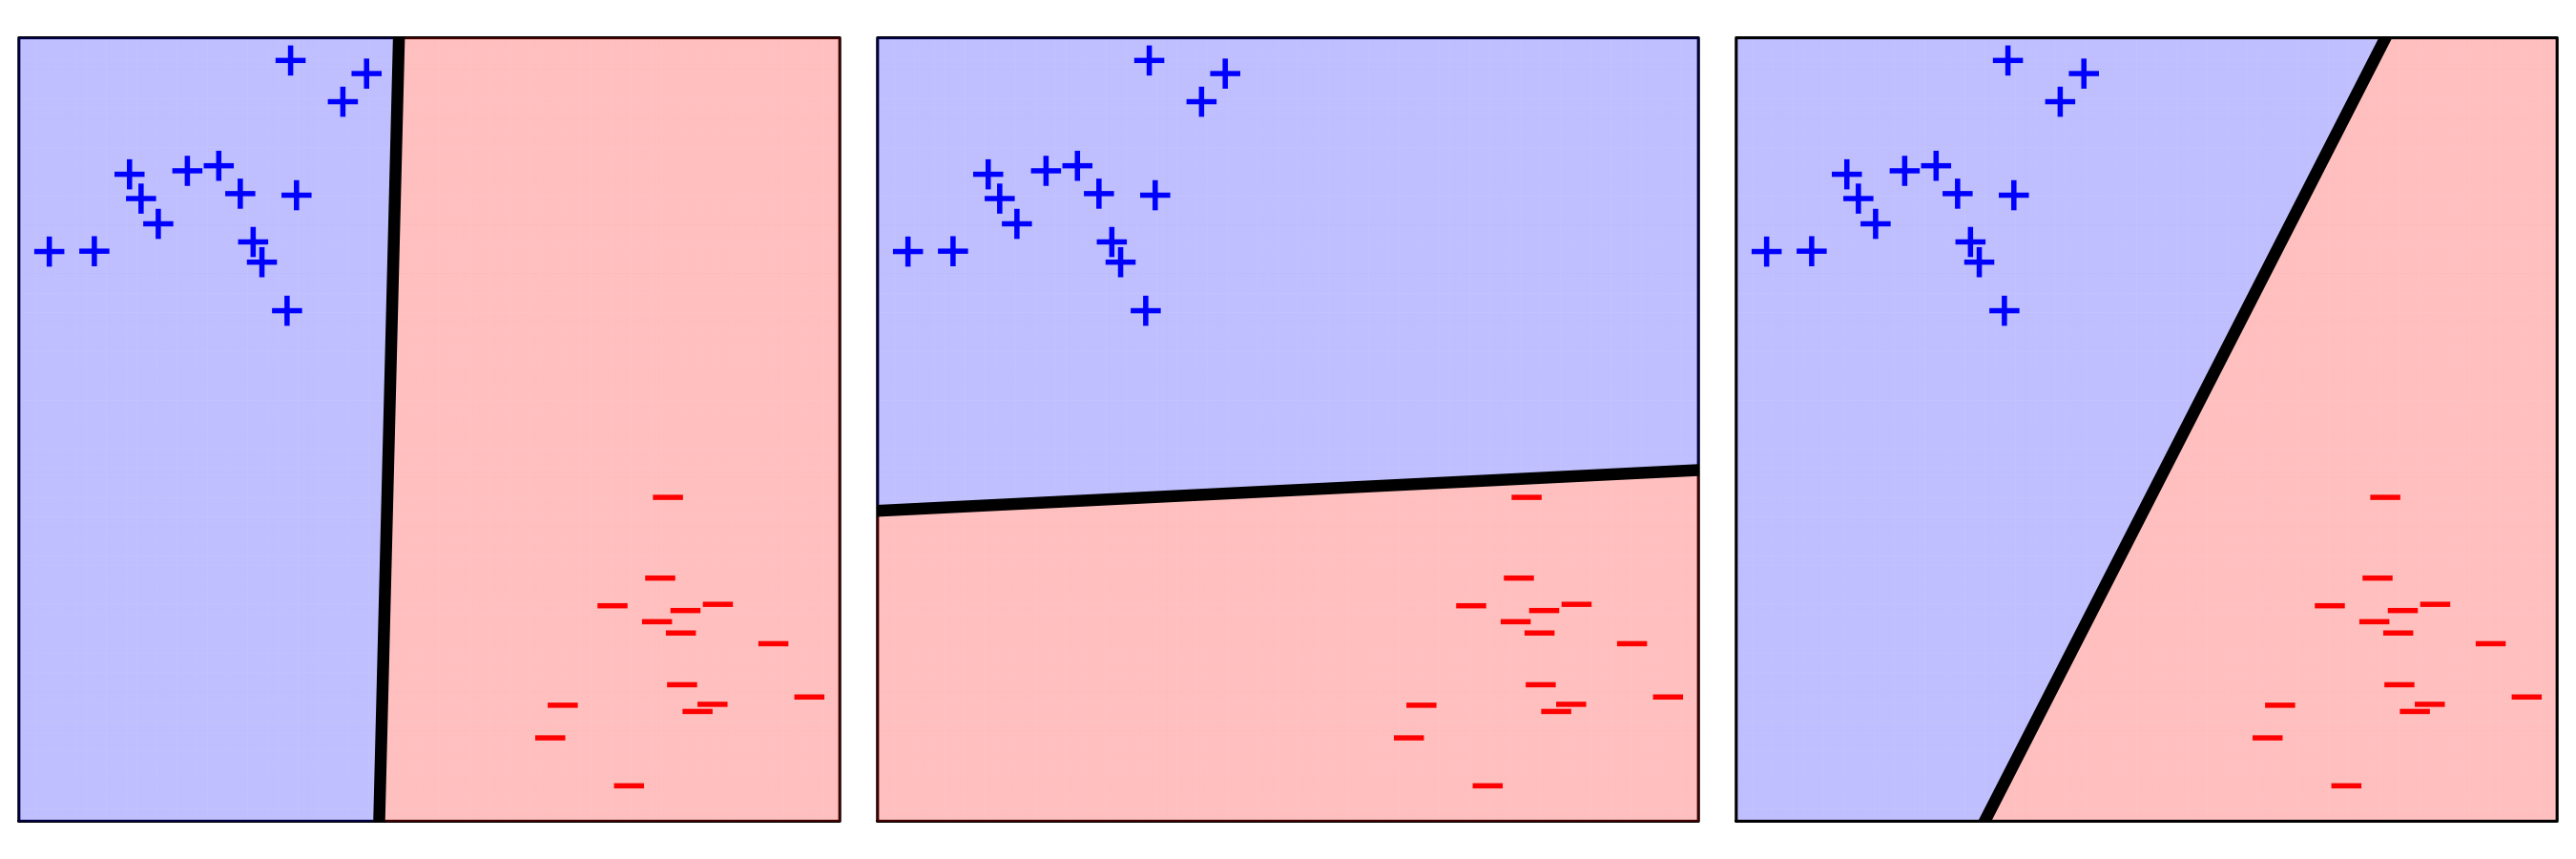
\includegraphics[width=\textwidth]{trennlinie.png}
\caption{M�gliche Hyperebenen zur Trennung der Trainingsdaten}
\label{possibleHP}
\end{figure}

\section{Entscheidungsfunktion}
%\subsection*{Entscheidungsfunktion}
Zun�chst wird begr�ndet, wie sich die Entscheidungsfunktion $f(\mathbf{x}) $ aus den Beobachtungen $\mathbf{x}$ zusammensetzt.
Dazu betrachtet man in Abbildung \ref{decisionfunction} die zwei Halbr�ume 
\begin{itemize}
\item $\mathbf{w}^\top \mathbf{x}+ b > 0$ (blau) und 
\item $\mathbf{w}^\top \mathbf{x}+ b < 0$ (rot),
\end{itemize}
die beim Trennen eines zweidimensionalen Variablenraums durch eine Hyperebene wie in Gleichung (\ref{hyperebene}) entstehen.
%Abbildung \ref{decisionfunction} visualisiert die zwei Halbr�ume $\mathbf{w}^\top \mathbf{x}+ b > 0$ (blau) und $\mathbf{w}^\top \mathbf{x}+ b < 0$ (rot), die beim trennen des 
%(in diesem Fall zweidimensionalen) 
%Variablenraums durch eine Hyperebene wie in Gleichung (\ref{hyperebene}) entstehen.
Mit Hilfe einer Entscheidungsfunktion $f(\mathbf{x})$ sollen
\begin{itemize}
\item Beobachtungen der positiven Klasse $y_i=+1$ in den Halbraum $\mathbf{w}^\top \mathbf{x}+ b > 0$ und
\item Beobachtungen der negativen Klasse $y_i=-1$ in den Halbraum $\mathbf{w}^\top \mathbf{x}+ b < 0$ 
\end{itemize} 
zugeordnet werden. Die Wahl von $f(\mathbf{x}) = \text{sgn}(\mathbf{w}^\top \mathbf{x}+ b)$ erm�glicht eine solche Zuordnung (vgl. \citealp[Kap. 2]{ben2010user}; \citealp[Kap. 7.1]{scholkopf2001learning}).

\begin{figure}[!h]
\centering
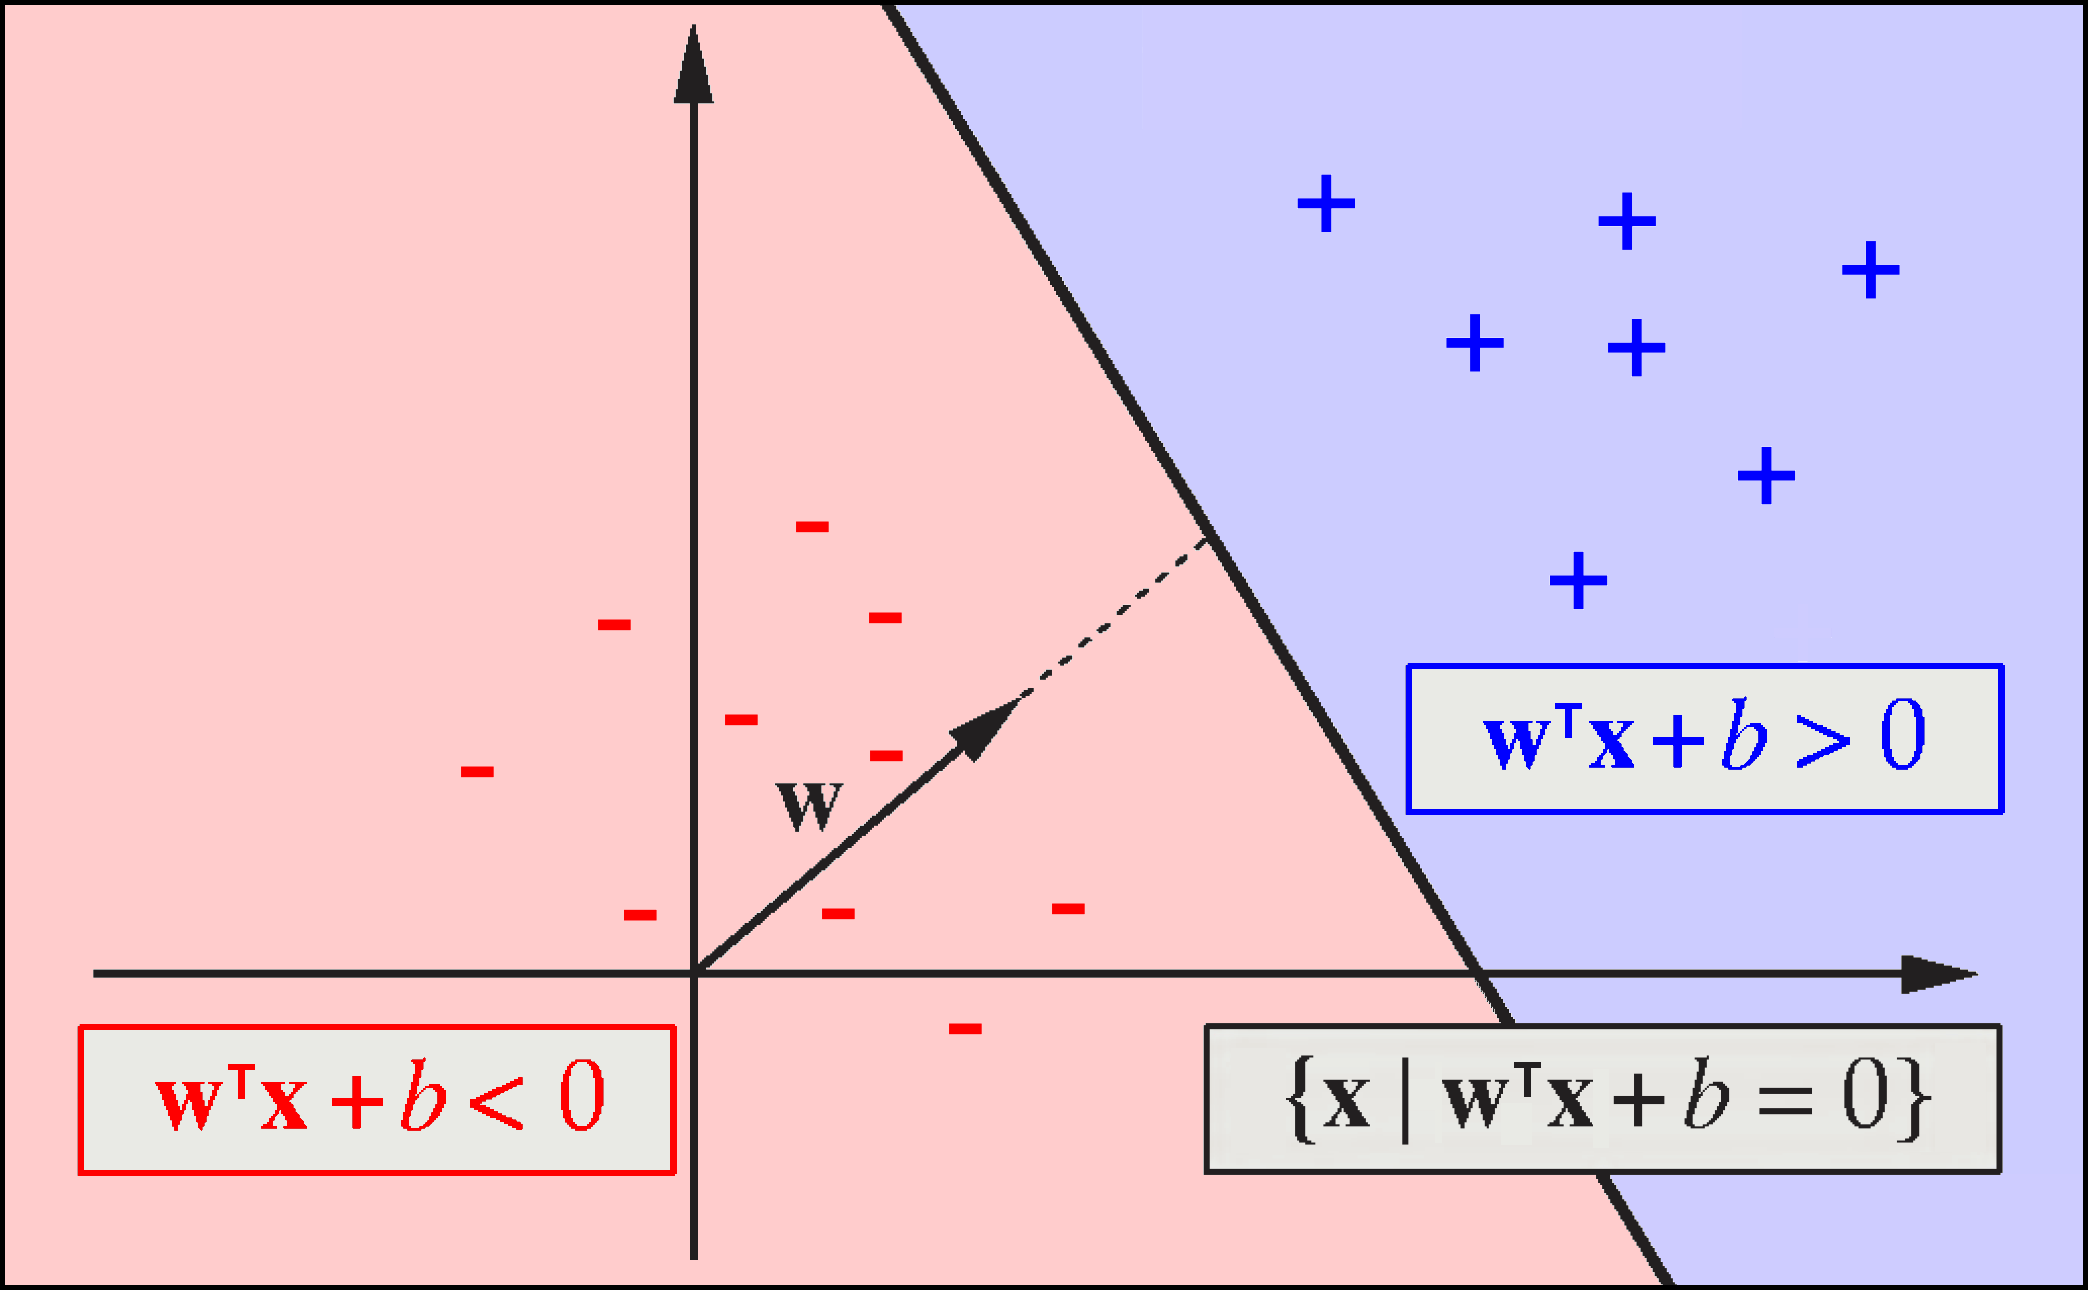
\includegraphics[width=0.8\textwidth]{hyperplane3.png}
\caption{Bereiche ``oberhalb'' und ``unterhalb'' der Hyperebene}
\label{decisionfunction}
\end{figure}

\section{Kanonische Hyperebene}

Die Hyperebene aus Gleichung (\ref{hyperebene}) ist invariant gegen�ber der Multiplikation mit einer beliebigen positiven Zahl $\lambda$. Die Lage und Position der Hyperebene bleibt wegen
%kann mit jeder beliebigen positiven Zahl $\lambda \in \mathbb{R}^+$ multiplizieren werden, wobei gleichzeitig die Form der Hyperebene unver�ndert bleibt. Es gilt
\begin{align*}
\mathbf{w}^\top \mathbf{x}+ b = 0 \;
\Leftrightarrow \; \lambda \mathbf{w}^\top \mathbf{x}+ \lambda b = 0,
\end{align*}
f�r alle $\lambda \in \mathbb{R}^+$ unver�ndert. Daraus resultiert das Problem, dass es unendlich viele Gleichungen gibt, welche dieselbe Hyperebene beschreiben. Um dies zu umgehen, f�hrt man eine sogenannte kanonische Hyperebene ein, die zus�tzlich die Einschr�nkung
\begin{equation*}
\label{kanonicalHP}
\min_{i=1, \hdots, N} | \mathbf{w}^\top \mathbf{x}_i + b | = 1
\end{equation*}
hat. Dadurch wird der Abstand der n�chstgelegenen Beobachtungen zur Hyperebene so skaliert, dass er betragsm��ig gleich $1$ ist. Dieser Abstand ist  
%nicht etwa als euklidischer Abstand interpretiert werden sondern 
als funktionaler Abstand zu interpretieren, der lediglich die Abst�nde einer Beobachtung relativ zu den n�chstgelegenen Beobachtungen zur Hyperebene wiedergibt. Alle anderen Beobachtungen haben demnach einen betragsm��igen funktionalen Abstand von der Hyperebene, der gr��er als $1$ ist. 
Es gilt
%\begin{align*}
%&\mathbf{w}^\top \mathbf{x}_i + b \geq +1 \; \text{ f�r } \; y_i = +1 \\
%&\mathbf{w}^\top \mathbf{x}_i + b \leq -1 \; \text{ f�r } \; y_i = -1,
%\end{align*}
$$
\left\{
  \begin{array}{ll}
	\mathbf{w}^\top \mathbf{x}_i + b \geq +1 &\text{f�r} \; y_i = +1 \\
	\mathbf{w}^\top \mathbf{x}_i + b \leq -1  &\text{f�r} \; y_i = -1,
  \end{array}
\right.
$$
beziehungsweise in kompakter Form $y_i (\mathbf{w}^\top \mathbf{x}_i + b) \geq 1$.
Diese Ungleichung gibt den betragsm��igen funktionalen Abstand einer Beobachtung $\mathbf{x}_i$ orthogonal zur Hyperebene an (\citealp[vgl.][Kap. 7.1]{scholkopf2001learning}).

Abbildung \ref{margin} veranschaulicht diesen Sachverhalt am Beispiel eines zweidimensionalen Variablenraums:
Die ausgef�llten Punkte auf den gestrichelten Geraden entsprechen den zur Hyperebene n�chstgelegenen Beobachtungen. Ihr funktionaler Abstand orthogonal zur Hyperebene betr�gt $1$. Sie werden St�tzvektoren (engl. \textit{support vectors}) genannt, da sie den Richtungsvektor $\mathbf{w}$ der Hyperebene festlegen. Eine Verschiebung dieser Punkte bewirkt, dass sich der Richtungsvektor $\mathbf{w}$ und somit die Lage und Position der Hyperebene �ndert (vgl. auch letzter Absatz in Kapitel \ref{Optimierungsproblem}). 
Die gestrichelten %zur Hyperebene parallelen 
Geraden, auf denen die St�tzvektoren liegen, definieren den sogenannten Rand (engl.  \textit{margin}). Durch Maximierung des Randes erm�glicht man, dass der Abstand der Hyperebene zu beiden Klassen m�glichst gro� wird.
Im n�chsten Kapitel ist das Ziel einen mathematischen Ansatz herzuleiten, der diesen Rand maximiert.

\begin{figure}[!h]
\centering
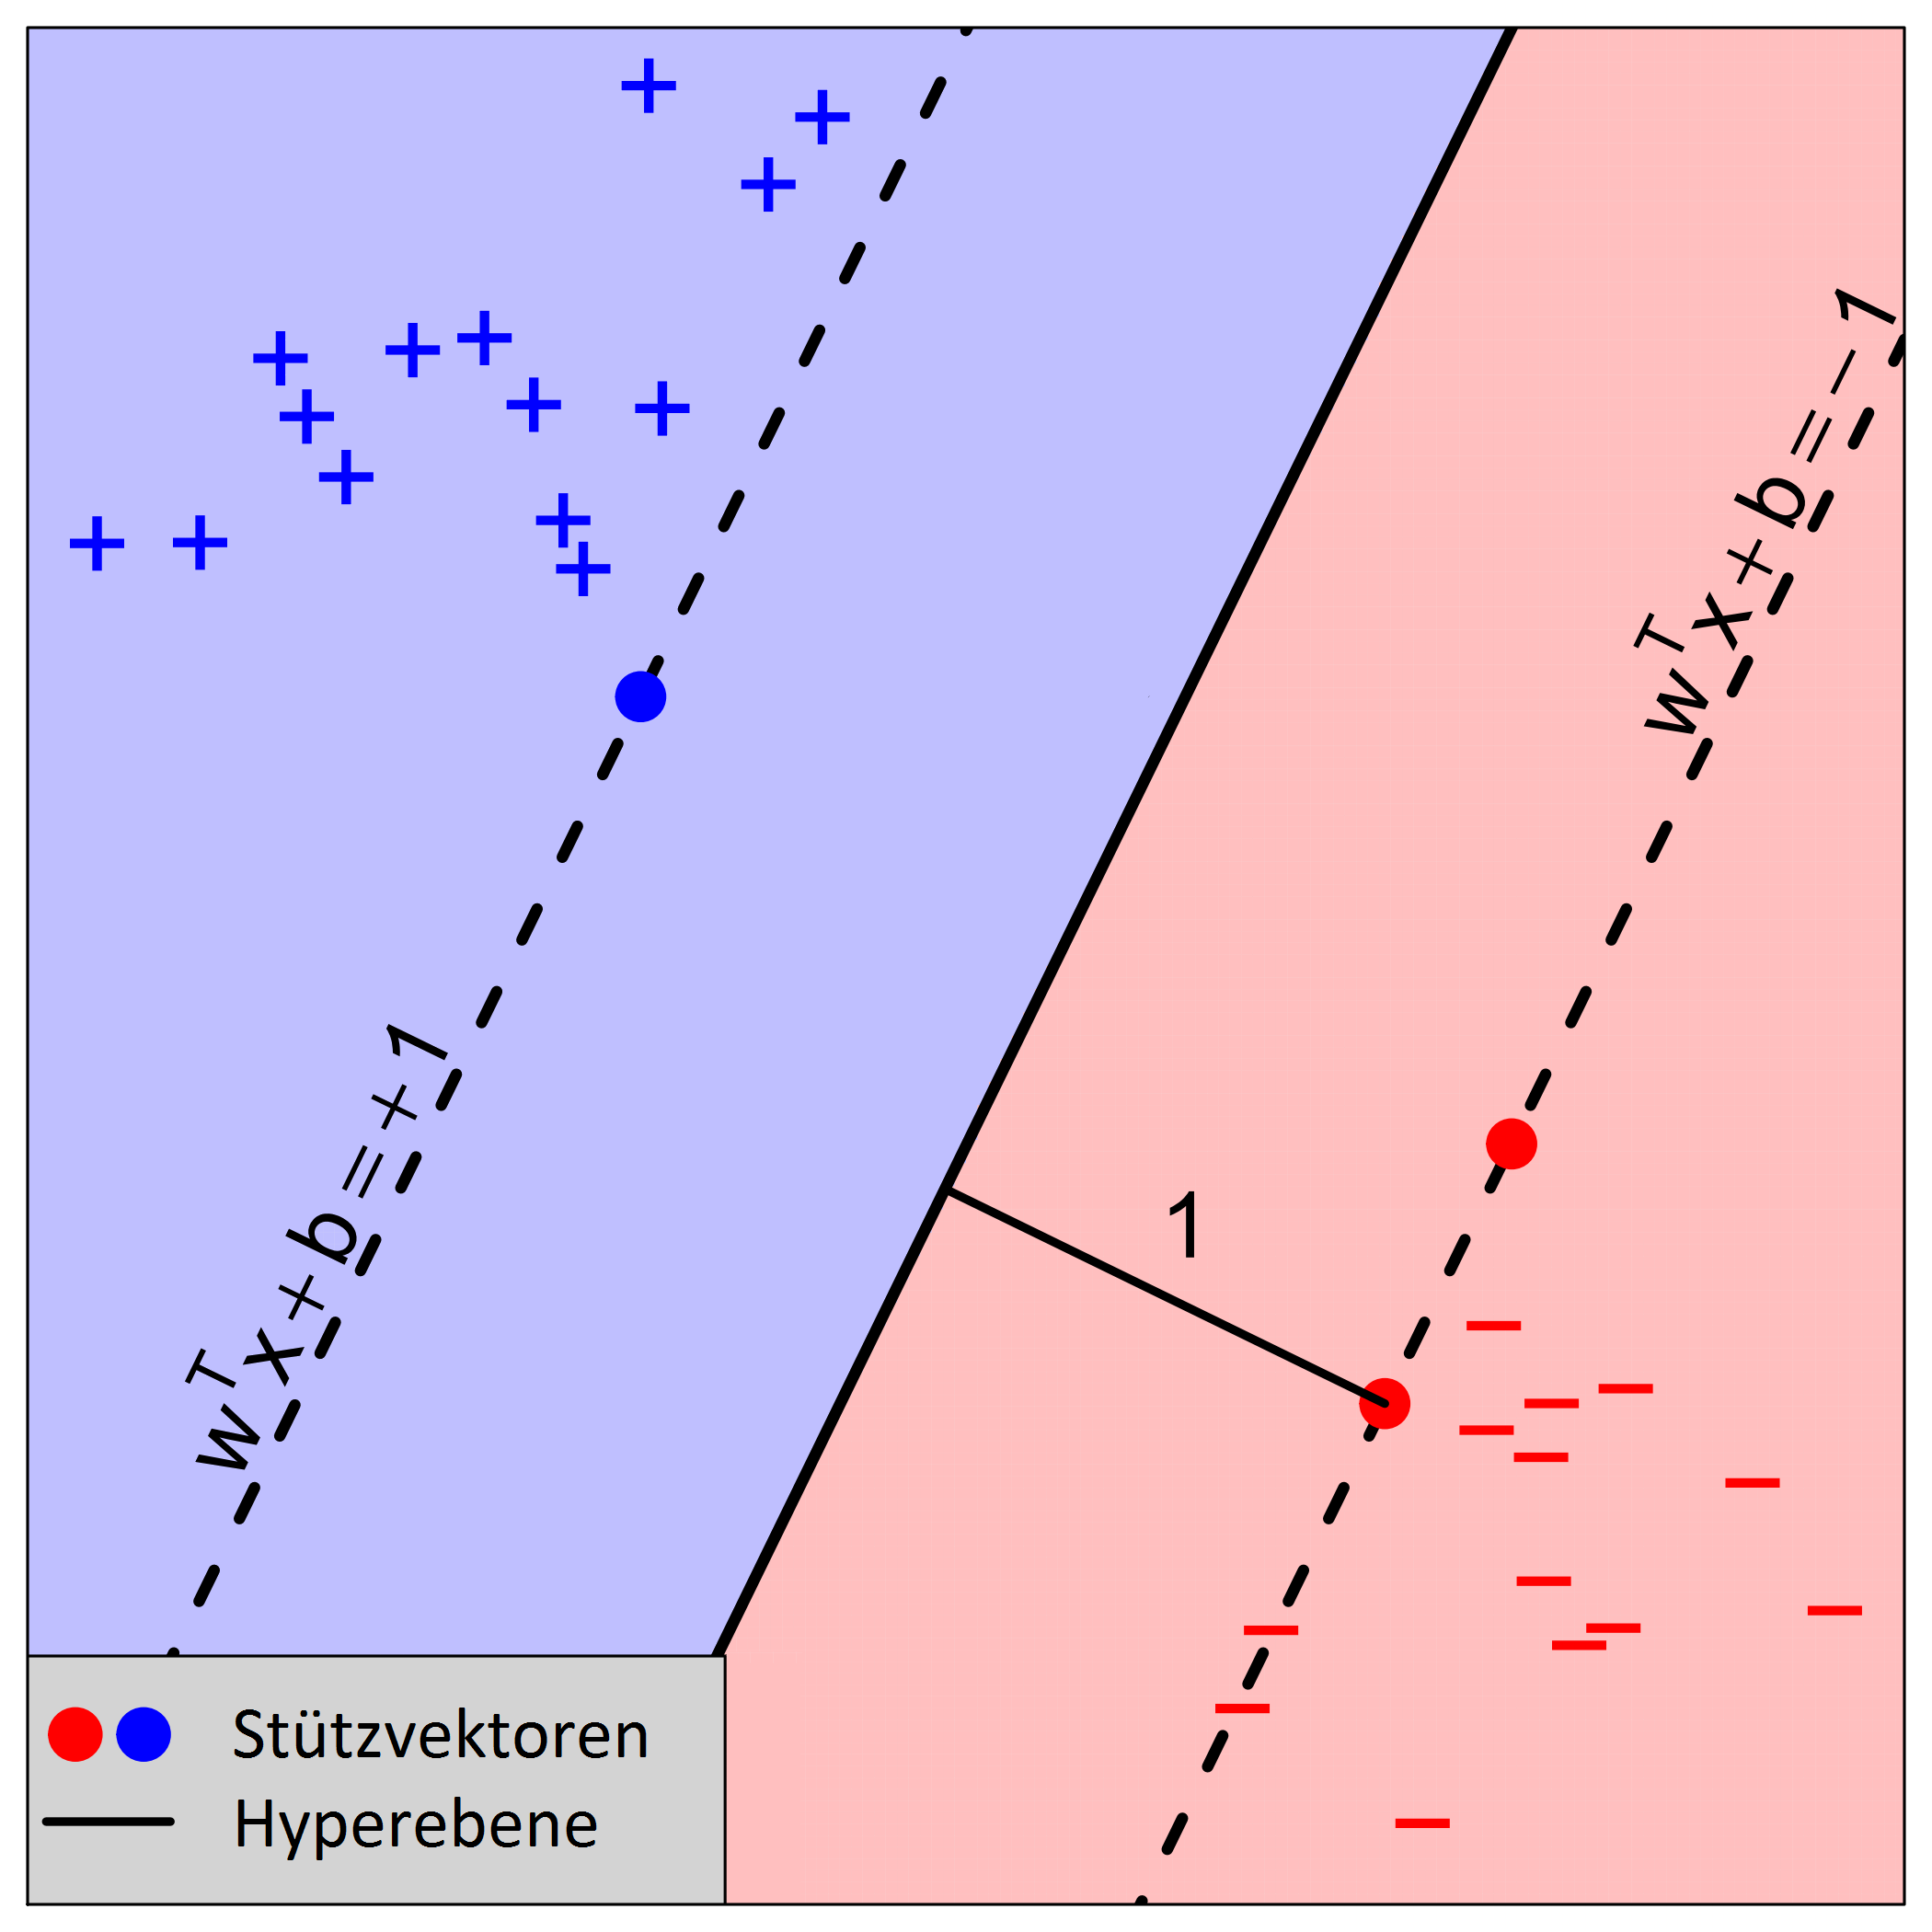
\includegraphics[width=0.6\textwidth]{margin3.png}
\caption{funktionale Abstand der St�tzvektoren zur Hyperebene betr�gt 1}
\label{margin}
\end{figure}

\section{Optimierungsproblem}
\label{Optimierungsproblem}
Die Hyperebene wird durch die bisher unbekannten Parameter $(\mathbf{w}, b)$ festgelegt. Um den euklidischen Abstand einer Beobachtung $\mathbf{x}_i$ orthogonal zur Hyperebene zu bestimmen, muss zus�tzlich mit der euklidischen Norm $||\mathbf{w}|| := \sqrt{\mathbf{w}^\top \mathbf{w}}$ normiert werden. Der euklidische Abstand berechnet sich durch
\begin{equation*}
d((\mathbf{w},b), \mathbf{x}_i) = \frac{y_i (\mathbf{w}^\top \mathbf{x}_i + b)}{||\mathbf{w}||} \geq \frac{1}{||\mathbf{w}||}.
\end{equation*}
%Die Support Vektoren haben also einen euklidischen Abstand von $\frac{1}{||\mathbf{w}||}$ von der Hyperebene (bzw. einen funktionalen Abstand von $1$). 
Um diesen euklidischen Abstand und somit den Rand zu maximieren, gen�gt es $||\mathbf{w}||$ bzw. $ \frac{1}{2} ||\mathbf{w}||^2$ zu minimieren (\citealp[vgl.][Kap. 3]{boswell2002introduction}).

Das daraus resultierende prim�re Optimierungsproblem lautet %kann wie folgt aufgestellt werden:
\begin{gather}
\begin{split}
\label{eq:nb}
& \min_{\mathbf{w},b} \hspace{8pt} \frac{1}{2} ||\mathbf{w}||^2\\
\text{NB:}          \hspace{8pt} & y_i (\mathbf{w}^\top \mathbf{x}_i + b) \geq 1,
\hspace{8pt} \forall i = 1, \hdots, N.
\end{split}
\end{gather}
Die dazugeh�rige Lagrange-Funktion mit Lagrange-Multiplikatoren $\alpha_i \geq 0$ hat die Form
\begin{align}
\label{primal}
L(\mathbf{w},b,\pmb{\alpha}) = \frac{1}{2} ||\mathbf{w}||^2 - \sum_{i=1}^{N} \alpha_i  (y_i (\mathbf{w}^\top \mathbf{x}_i + b) - 1).
\end{align}
In der Literatur wird aus praktischen Gr�nden das duale Optimierungsproblem bevorzugt. Um dieses herzuleiten, wird  die Lagrange-Funktion $L(\mathbf{w},b,\pmb{\alpha})$ bez�glich der Prim�rvariablen $\mathbf{w},b$ minimiert und bez�glich $\pmb{\alpha}$ maximiert (\citealp[vgl.][Kap. 7.3]{scholkopf2001learning}; \citealp[Kap. 5]{boyd2004convex}). 

F�r das Minimieren bez�glich der Prim�rvariablen ergeben sich folgende L�sungen (vgl. \citealp[S. 8]{gunn1998support}):
\begin{align}
\label{primal1}
\frac{\partial L(\mathbf{w},b,\pmb{\alpha})}{\partial b} = 0          & \Rightarrow \sum_{i=1}^N \alpha_i y_i = 0 \\
\label{primal2}
\frac{\partial L(\mathbf{w},b,\pmb{\alpha})}{\partial \mathbf{w}} = 0 & \Rightarrow \mathbf{w} = \sum_{i=1}^N \alpha_i y_i \mathbf{x}_i
\end{align}
Setzt man Gleichung (\ref{primal1}) und (\ref{primal2}) in die Lagrange-Funktion (\ref{primal}) ein, erh�lt man die sogenannte Lagrange-duale Funktion 
%$W(\pmb{\alpha}) = \min_{\mathbf{w}, b} L(\mathbf{w},b,\pmb{\alpha})$
\begin{align*}
W(\pmb{\alpha}) &=\min_{\mathbf{w}, b} L(\mathbf{w},b,\pmb{\alpha}) = \min_{\mathbf{w}, b} \left (\frac{1}{2} \mathbf{w}^\top \mathbf{w} - \sum_{i=1}^N \alpha_i (y_i ( \mathbf{w}^\top \mathbf{x}_i  +b) - 1) \right ) \\
&\stackrel{ (\ref{primal2})}= \min_{b} \left ( \frac{1}{2} \sum_{i=1}^N \alpha_i y_i \mathbf{x}_i^\top \sum_{j=1}^N \alpha_j y_j \mathbf{x}_j - \sum_{i=1}^N \alpha_i y_i \left ( \sum_{j=1}^N \alpha_j y_j \mathbf{x}_j^\top \right ) \mathbf{x}_i - \sum_{i=1}^N b \alpha_i y_i + \sum_{i=1}^N \alpha_i \right ) \\
&\stackrel{(\ref{primal1})}= \frac{1}{2} \sum_{i=1}^N \alpha_i y_i \mathbf{x}_i^\top \sum_{j=1}^N \alpha_j y_j \mathbf{x}_j - \sum_{i=1}^N \alpha_i y_i \left ( \sum_{j=1}^N \alpha_j y_j \mathbf{x}_j^\top \right ) \mathbf{x}_i + \sum_{i=1}^N \alpha_i \\
&=\frac{1}{2} \sum_{i,j=1}^N \alpha_i \alpha_j y_i y_j \mathbf{x}_i^{\top} \mathbf{x}_j - \sum_{i,j=1}^N \alpha_i \alpha_j y_i y_j \mathbf{x}_i^{\top} \mathbf{x}_j + \sum_{i=1}^N \alpha_i \\
&= -\frac{1}{2} \sum_{i,j=1}^N \alpha_i \alpha_j y_i y_j \mathbf{x}_i^{\top} \mathbf{x}_j + \sum_{i=1}^N \alpha_i.
\end{align*}
%Diese ist nicht mehr von den Prim�rvariablen $\mathbf{w},b$ abh�ngig. 
Das duale Optimierungsproblem ist nicht mehr von den Prim�rvariablen $\mathbf{w},b$ abh�ngig und l�sst sich wie folgt aufstellen (vgl. \citealp[S. 8]{gunn1998support}): 
\begin{gather}
\begin{split}
\label{dual}
\max_{\pmb{\alpha}} W(\pmb{\alpha}) = \max_{\pmb{\alpha}} 
\left ( \sum_{i=1}^N \alpha_i - \frac{1}{2} \sum_{i,j=1}^N \alpha_i \alpha_j y_i y_j \mathbf{x}_i^{\top} \mathbf{x}_j \right )\\
\text{NB:} \hspace{15pt} \alpha_i \geq 0, \hspace{20pt} \sum_{i=1}^N \alpha_i y_i = 0,  \hspace{20pt} \forall i= 1, \hdots, N
\end{split}
\end{gather}
Nach den Karush-Kuhn-Tucker (KKT) Bedingungen m�ssen alle Beobachtungen zus�tzlich die Bedingung $$\alpha_i [ y_i (\mathbf{w}^\top \mathbf{x}_i + b) -1 ] = 0 \hspace{8pt}$$
%\begin{align}
%\label{kkt}
%\alpha_i [ y_i (\mathbf{w}^\top \mathbf{x}_i + b) -1 ] = 0 \hspace{8pt} \forall i= 1, \hdots, N
%\end{align}
erf�llen (\citealp[vgl.][S. 197ff]{scholkopf2001learning}; \citealp[S. 4]{boswell2002introduction}). Dies impliziert, dass f�r alle Beobachtungen entweder $\alpha_i=0$ oder $y_i (\mathbf{w}^\top \mathbf{x}_i + b) = 1$ gelten muss.

\begin{itemize}
\item[$\pmb{\Rightarrow}$] $\alpha_i=0$, wenn $y_i (\mathbf{w}^\top \mathbf{x}_i + b) > 1$, d.h. wenn der funktionale Abstand einer Beobachtung $\mathbf{x}_i$ zur Hyperebene gr��er als $1$ ist. %In Abbildung \ref{margin} sind das diejenigen Beobachtungen, die nicht auf den gestrichelten Geraden liegen.

\item[$\pmb{\Rightarrow}$] Es interessieren nur die St�tzvektoren, da f�r diese $ y_i (\mathbf{w}^\top \mathbf{x}_i + b) = 1$ gilt, d.h. der funktionale Abstand eines St�tzvektors zur Hyperebene betr�gt $1$.
\end{itemize}

F�r die Berechnung der Hyperebenenparameter $(\mathbf{w}, b)$ sind deshalb nur die St�tzvektoren n�tig. F�r alle anderen Beobachtungen $\mathbf{x}_i$ sind die dazugeh�rigen $\alpha_i = 0$ und bleiben deshalb bei der Berechnung von $\mathbf{w} = \sum_{i=1}^N \alpha_i y_i \mathbf{x}_i$ unber�cksichtigt. Somit ist der Parameter $\mathbf{w}$ lediglich eine Linearkombination der St�tzvektoren.
Der Parameter $b$ kann aus der Gleichung 
\begin{align*}
y_j = \mathbf{w}^\top \mathbf{x}_j + b = \sum_{i=1}^N \alpha_i y_i \mathbf{x}_i^\top  \mathbf{x}_j + b \;
\Leftrightarrow \; b = y_j - \sum_{i=1}^N \alpha_i y_i \mathbf{x}_i^\top  \mathbf{x}_j
\end{align*}
ermittelt werden. Die Entscheidungsfunktion zur Klassifizierung einer Beobachtung $\mathbf{x}_j$ lautet $$f(\mathbf{x}_j) = \text{sgn} \left (\mathbf{w}^\top \mathbf{x}_j + b \right ) =  \text{sgn} \left (\sum_{i=1}^N \alpha_i y_i \mathbf{x}_i^\top \mathbf{x}_j  + b \right ).$$

%Der Parameter $b$ f�r die Verschiebung der Hyperebene kann aus ein Support Vektor der positiven Klasse $\mathbf{x}^{+}$ und ein Support Vektor der negativen Klasse $\mathbf{x}^{-}$ mit den Gleichungen
%\begin{align*}
%\mathbf{w}^{\top} \mathbf{x}^{+} + b = +1\\
%\mathbf{w}^{\top} \mathbf{x}^{-} + b = -1
%\end{align*}
%berechnet werden. Aufsummieren beider Gleichungen ergibt $b= - \tfrac{1}{2} ( \mathbf{w}^{\top} \mathbf{x}^{+} +  \mathbf{w}^{\top} \mathbf{x}^{-})$.


%\section{Zusammenfassung}



\chapter{Nicht linear trennbare Daten}
\label{chap:nichttrennbar}

\section{Kern Trick}
\label{sec:kerneltrick}
Bisher wurde angenommen, dass die Daten linear trennbar sind. Dies ist in der Praxis nicht immer der Fall. Eine M�glichkeit mit nicht linear trennbaren Daten umzugehen ist der sogenannte Kern Trick. Hierbei ist die Idee, die Daten mit Hilfe einer Funktion $\Phi$ in einen h�herdimensionalen Variablenraum zu �berf�hren, in dem sie linear trennbar sind.

Auf der linken Seite von Abbildung \ref{kerntrick} ist ein solcher nicht linear trennbarer Fall in einem zweidimensionalen Variablenraum $\mathbf{x} = (x_1,x_2)$ dargestellt.
%Die Daten sind hier nicht durch eine Gerade, sondern durch eine Ellipse trennbar. 
%Man kann im vorliegenden zweidimensionalen Variablenraum keine Hyperebene (Gerade) legen,
Hierbei kann keine Hyperebene (hier Gerade) gefunden werden, 
so dass die roten Punkte von den blauen Kreuzen vollst�ndig getrennt werden. 
%Allerdings lassen sich die Daten 
Durch geschickte Wahl von $\Phi$ lassen sich die Daten in einen dreidimensionalen Variablenraum �berf�hren, indem sie sich durch eine Hyperebene (hier Ebene) linear trennen lassen.
%Um genauer auf die Situation aus Abbildung \ref{kerntrick} einzugehen, wird die Funktion
Dies geschieht beispielsweise mit der Wahl von
\begin{equation}
\label{phi}
\Phi(\mathbf{x}) = \Phi((x_1,x_2)) = (x_1^2, x_2^2, \sqrt{2}x_1 x_2),
%\begin{array}{ccccc}
%\Phi: & \mathbb{R}^2   & \rightarrow & \mathbb{R}^3 & \\
%      & (x_1,x_2)      & \rightarrow & (x_1^2,\sqrt{2}x_1 x_2, x_2^2)  & =: (z_1,z_2,z_3) = \mathbf{z}^{\top}
%\end{array}
\end{equation}
womit der zweidimensionale Variablenraum in einen dreidimensionalen Variablenraum �berf�hrt wird, d.h. $\Phi: \mathbb{R}^2 \rightarrow \mathbb{R}^3$.
%Durch diese Wahl von $\Phi$ wird im folgenden gezeigt, dass im h�herdimensionalen Variablenraum 
%(hier dreidimensionaler Variablenraum, da $(x_1^2, x_2^2, \sqrt{2}x_1 x_2) \in \mathbb{R}^3$)
% die Daten linear trennbar sind, w�hrend sie im zweidimensionalen Variablenraum durch eine Ellipse getrennt werden. 
Die linear trennende Hyperebene im $\mathbb{R}^3$ hat die Form
\begin{align}
\label{rhochdrei} 
                & \; \mathbf{w}^\top \Phi(\mathbf{x}) + b =  0 \\
\Leftrightarrow & \; \mathbf{w}^\top (x_1^2, x_2^2, \sqrt{2}x_1 x_2) + b =  0 \notag \\
\label{ellipsengleichung} 
\Leftrightarrow & \; w_1 x_1^2 + w_2 x_2^2 + w_3 \sqrt{2}x_1 x_2 + b= 0.
\end{align}
Durch Einsetzen von Gleichung (\ref{phi}) in die Hyperebenengleichung (\ref{rhochdrei}) resultiert die Gleichung (\ref{ellipsengleichung}). Diese entspricht genau der Gleichung eines Kegelschnitts, was z.B. eine Hyperbel oder Ellipse im $\mathbb{R}^2$ sein kann (\citealp[vgl.][Kap. 3]{ben2010user}). Durch die obige Wahl von $\Phi$, k�nnen Daten, die im zweidimensionalen Variablenraum durch eine Ellipse trennbar sind, in einen dreidimensionalen Variablenraum durch eine Ebene linear getrennt werden.
%Deshalb k�nnen durch obige Wahl von $\Phi$ die im zweidimensionalen Variablenraum durch eine Ellipse trennbare Daten, in einem dreidimensionalen Variablenraum durch eine Ebene linear getrennt werden.
%TODO: Mengen die aus einem Punkt bestehen im 1 dim, Gerade im 2 dim, Ebene im 3 dim
%TODO: Zitat von Gleichungen in Klammern
%TODO: $w^\top x_i$ mit eckiger Schreibwesie ersetzen
%Zugegeben ist die Wahl von $\Phi$ nicht immer einfach. 
%Man kann allgemein zeigen, dass durch Wahl einer geeigneten Kernfunktion $K$ die Funktion $\Phi$ festgelegt wird. QUELLE
Die Wahl von $\Phi$ kann in der Praxis wegen Skalarproduktberechnungen im h�herdimensionalen Raum der Form $\Phi(\mathbf{x}_i)^\top \Phi(\mathbf{x}_j) $ sehr rechenintensiv sein. Deshalb verwendet man h�ufig eine sogenannte Kernfunktion $K(\mathbf{x}_i, \mathbf{x}_j)$, welche die Funktion $\Phi$ implizit festlegt und meist auf Skalarproduktberechnungen im niedrigdimensionalen Raum beruht. Beispielsweise beruht die polynomiale Kernfunktion auf Skalarproduktberechnungen der Form $\mathbf{x}_i^\top \mathbf{x}_j$. In der Literatur werden im Allgemeinen die folgenden Kernfunktionen genannt (\citealp[vgl.][Kap. 3.1]{gunn1998support}; \citealp[Kap. 7.4]{scholkopf2001learning}):

\begin{figure}[t]
\label{kerntrick}
\centering
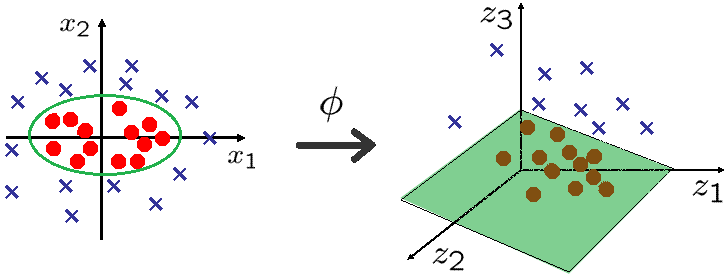
\includegraphics[width=\textwidth]{bild3}
\caption{�berf�hrung eines zweidimensionalen Variablenraums in einen h�herdimensionalen (hier dreidimensionalen) Variablenraum, in dem die Daten linear trennbar sind. Dabei gilt $(z_1,z_2,z_3) := (x_1^2, x_2^2, \sqrt{2}x_1 x_2)$. }
\end{figure}

\begin{itemize}
\item polynomiale Kernfunktion vom Grad $d$: $K(\mathbf{x}_i,\mathbf{x}_j) = (\mathbf{x}_i^\top \mathbf{x}_j + c) ^d $ mit $c \in \{0,1\}$
\item gau�sche radiale Basisfunktion: $K(\mathbf{x}_i,\mathbf{x}_j) = \exp{ \left ( -\frac{||\mathbf{x}_i - \mathbf{x}_j ||}{c} \right ) }$, f�r $c > 0$.
\end{itemize}

%F�r jede Beobachtung errechnet man mittels $\Phi$ aus den alten Variablen neue Variablen. In diesem neuen Variablenraum sind die Beobachtungen linear trennbar.
%$\Phi$ wird dabei durch eine Kernfunktion festgelegt. Die Kernfunktion verh�lt sich im �berf�hrten h�herdimensionalen Raum wie ein Skalarprodukt, d.h.

Dabei sind $c$ und $d$ Kern-Parameter, die durch Kreuzvalidierung bestimmt werden k�nnen. F�r eine Kernfunktion gilt stets 
\begin{equation}
\label{eq:kernel}
K(\mathbf{x}_i, \mathbf{x}_j) = \Phi(\mathbf{x}_i)^\top \Phi(\mathbf{x}_j) .
\end{equation}
Das folgende Beispiel zeigt, dass eine polynomiale Kernfunktion vom Grad $d=2$ 
mit $c=0$
die Gleichung (\ref{eq:kernel}) erf�llt und zugleich die implizit festgelegte Funktion $\Phi$ identisch zu Gleichung (\ref{phi}) ist. Dabei werden Beobachtungen mit zwei Variablen, d.h. $\mathbf{x}_i = (x_{i_1}, x_{i_2}), \; i=1,2$ betrachtet:
\begin{align*}
K({\color{red}\mathbf{x}_1},\mathbf{x}_2) 
           &= ({\color{red}\mathbf{x}_1}^\top \mathbf{x}_2 )^2 = ( {\color{red}(x_{1_1},x_{1_2})}^\top (x_{2_1},x_{2_2}) )^2\\
           &= ({\color{red}x_{1_1}}x_{2_1} + {\color{red}x_{1_2}}x_{2_2})^2 \\
           &= ({\color{red}x_{1_1}^2} x_{2_1}^2  + {\color{red}x_{1_2}^2} x_{2_2}^2 + 2{\color{red}x_{1_1} x_{1_2}}x_{2_1}x_{2_2})\\
           &= ({\color{red}x_{1_1}^2}, {\color{red}x_{1_2}^2}, {\color{red} \sqrt{2} x_{1_1} x_{1_2}})^\top
              (x_{2_1}^2, x_{2_2}^2, \sqrt{2} x_{2_1} x_{2_2}) \\
           &= \Phi({\color{red}\mathbf{x}_1})^\top \Phi(\mathbf{x}_2)  
           & \Rightarrow \Phi(\mathbf{x}) = (x_1^2, x_2^2, \sqrt{2}x_1 x_2)
\end{align*}
%Die Wahl einer polynomialen Kernfunktion vom Grad $d=2$ mit $c=0$ entspricht also der gleichen Situation aus Gleichung \ref{phi}.
%Abbildung \ref{kerntrick}, wobei die Funktion $\Phi$ die gleiche Form aus Gleichung \ref{phi} hat.
%Der einzige Unterschied zum vorherigen Kapitel ist hier, dass man den Merkmalsvektor $\mathbf{x}_i$ mit dem h�herdimensionalen Merkmalsvektor $\Phi(\mathbf{x}_i)$ ersetzt. Die Entscheidungsfunktion lautet dann
Ein Beweis, dass die Gleichung (\ref{eq:kernel}) auch f�r allgemeine polynomiale Kernfunktionen vom Grad $d$ mit den Konstanten $c=0$ bzw. $c=1$ und f�r die gau�sche radiale Basisfunktion gilt, kann in \citet[Kap. 2]{scholkopf2001learning} bzw. \citet[Kap. 5.8]{hastie2011elements} nachgeschlagen werden.

Das weitere Vorgehen zur Bestimmung der Hyperebenenparameter $\mathbf{w},b$) ist analog zum Kapitel \ref{Optimierungsproblem}. Der einzige Unterschied ist, dass man den Merkmalsvektor $\mathbf{x}_i$ mit den h�herdimensionalen Merkmalsvektor $\Phi(\mathbf{x}_i)$ ersetzt und bei Skalarproduktberechnungen der Form $ \Phi(\mathbf{x}_i)^\top \Phi(\mathbf{x}_j)$ eine Kernfunktion $K(\mathbf{x}_i,\mathbf{x}_j)$ verwendet. Als Entscheidungsfunktion f�r eine Beobachtung $\mathbf{x}_j$ ergibt sich somit
%$$f(\mathbf{x}) = \sgn \left ( \sum_{i=1}^N y_i \alpha_i {\color{red} \langle \mathbf{x}_i, \mathbf{x} \rangle} + b \right )$$
%verwendet wird, sondern  
$$f(\mathbf{x}_j) = \sgn \left ( \sum_{i=1}^N y_i \alpha_i {\color{red} \Phi(\mathbf{x}_i)^\top \Phi(\mathbf{x}_j)} + b \right ) = \sgn \left ( \sum_{i=1}^N y_i \alpha_i {\color{red}K(\mathbf{x}_i,\mathbf{x}_j)} + b \right ).$$

\section{Soft Margin}
\label{sec:softmargin}
%Beim Kern-Trick k�nnen bereits einzelne Ausreiser in den Daten die Form der Hyperebene stark beeinflussen, so dass es sinnvoll ist
Bisher wird durch die Nebenbedingung $y_i (\mathbf{w}^\top \mathbf{x}_i + b) \geq 1$ aus Gleichung (\ref{eq:nb}), beziehungsweise beim Kern-Trick die Nebenbedingung $y_i (\mathbf{w}^\top \Phi(\mathbf{x}_i) + b) \geq 1$, gew�hrleistet, dass die Daten durch eine Hyperebene vollst�ndig getrennt werden und man somit Fehlklassifizierungen vermeidet. Bei Ausrei�ern in den Daten kann dies zu Overfitting f�hren. Daher ist es w�nschenswert Fehlklassifizierung zu erlauben, diese aber entsprechend zu bestrafen.
%Dies ist auch beim Kern-Trick der Fall, da hier durch die �berf�hrung des Merkmalsvektors in einen h�herdimensionalen Merkmalsvektor eine flexible Trennung der beiden Klassen erm�glicht. 
%Zur Veranschaulichung ist in Abbildung \ref{fig:kerntrick} und Abbildung \ref{fig:softmargin} zwei mal die gleiche Datensitation dargestellt. 
In Abbildung \ref{fig:kerntrick} werden die Daten mit dem Kern Trick vollst�ndig voneinander getrennt. 
Neue Beobachtungen auf der oberen linken Ecke w�rden hier in die negative (rote) Klasse klassifiziert werden, obwohl eine Klassifizierung in die positive (blaue) Klasse sinnvoller erscheint. Betrachtet man die gr�n eingekreisten Beobachtungen als Ausrei�er, kann man deshalb hier von einem Overfittig ausgehen.
%Die Soft Margin Hyperebene in Abbildung \ref{fig:softmargin} kann bei der gleichen Datensitation hier sinnvoller sein. 
Die Soft Margin Hyperebene in Abbildung \ref{fig:softmargin} entsch�rft die oben erw�hnte Nebenbedingung, so dass f�r einzelne Ausrei�er eine Fehlklassifizierung erlaubt wird. Dies geschieht mit sogenannten Schlupfvariablen (engl. \textit{slack variables}) $\xi_i \geq 0$. Die entsch�rfte Nebenbedingung lautet 
$$y_i (\mathbf{w}^\top \mathbf{x}_i + b) \geq 1 - \xi_i, \; i=1,\hdots, N$$
und erm�glicht, dass sich einige Beobachtungen innerhalb des Randes oder auf der falschen Seite der Hyperebene befinden d�rfen. In Abbildung \ref{fig:softmargin} sind das die mit $\xi_1, \hdots, \xi_5$ gekennzeichneten Beobachtungen. Dabei gibt $\xi_i$ die Entfernung zwischen Beobachtung und der entsprechenden gestrichelten Linie an. Die Beobachtungen sind f�r

\begin{itemize}
\item $\xi_i = 0$ richtig klassifiziert, %e Trainingsdaten
\item $0<\xi_i \leq 1$ innerhalb des Randes richtig klassifiziert und
\item $\xi_i > 1$ fehlklassifiziert \cite[Kap. 4.2]{ben2010user}. %e Trainingsdaten
\end{itemize}

\begin{figure}[ht]
\begin{minipage}[b]{0.5\linewidth}
\centering
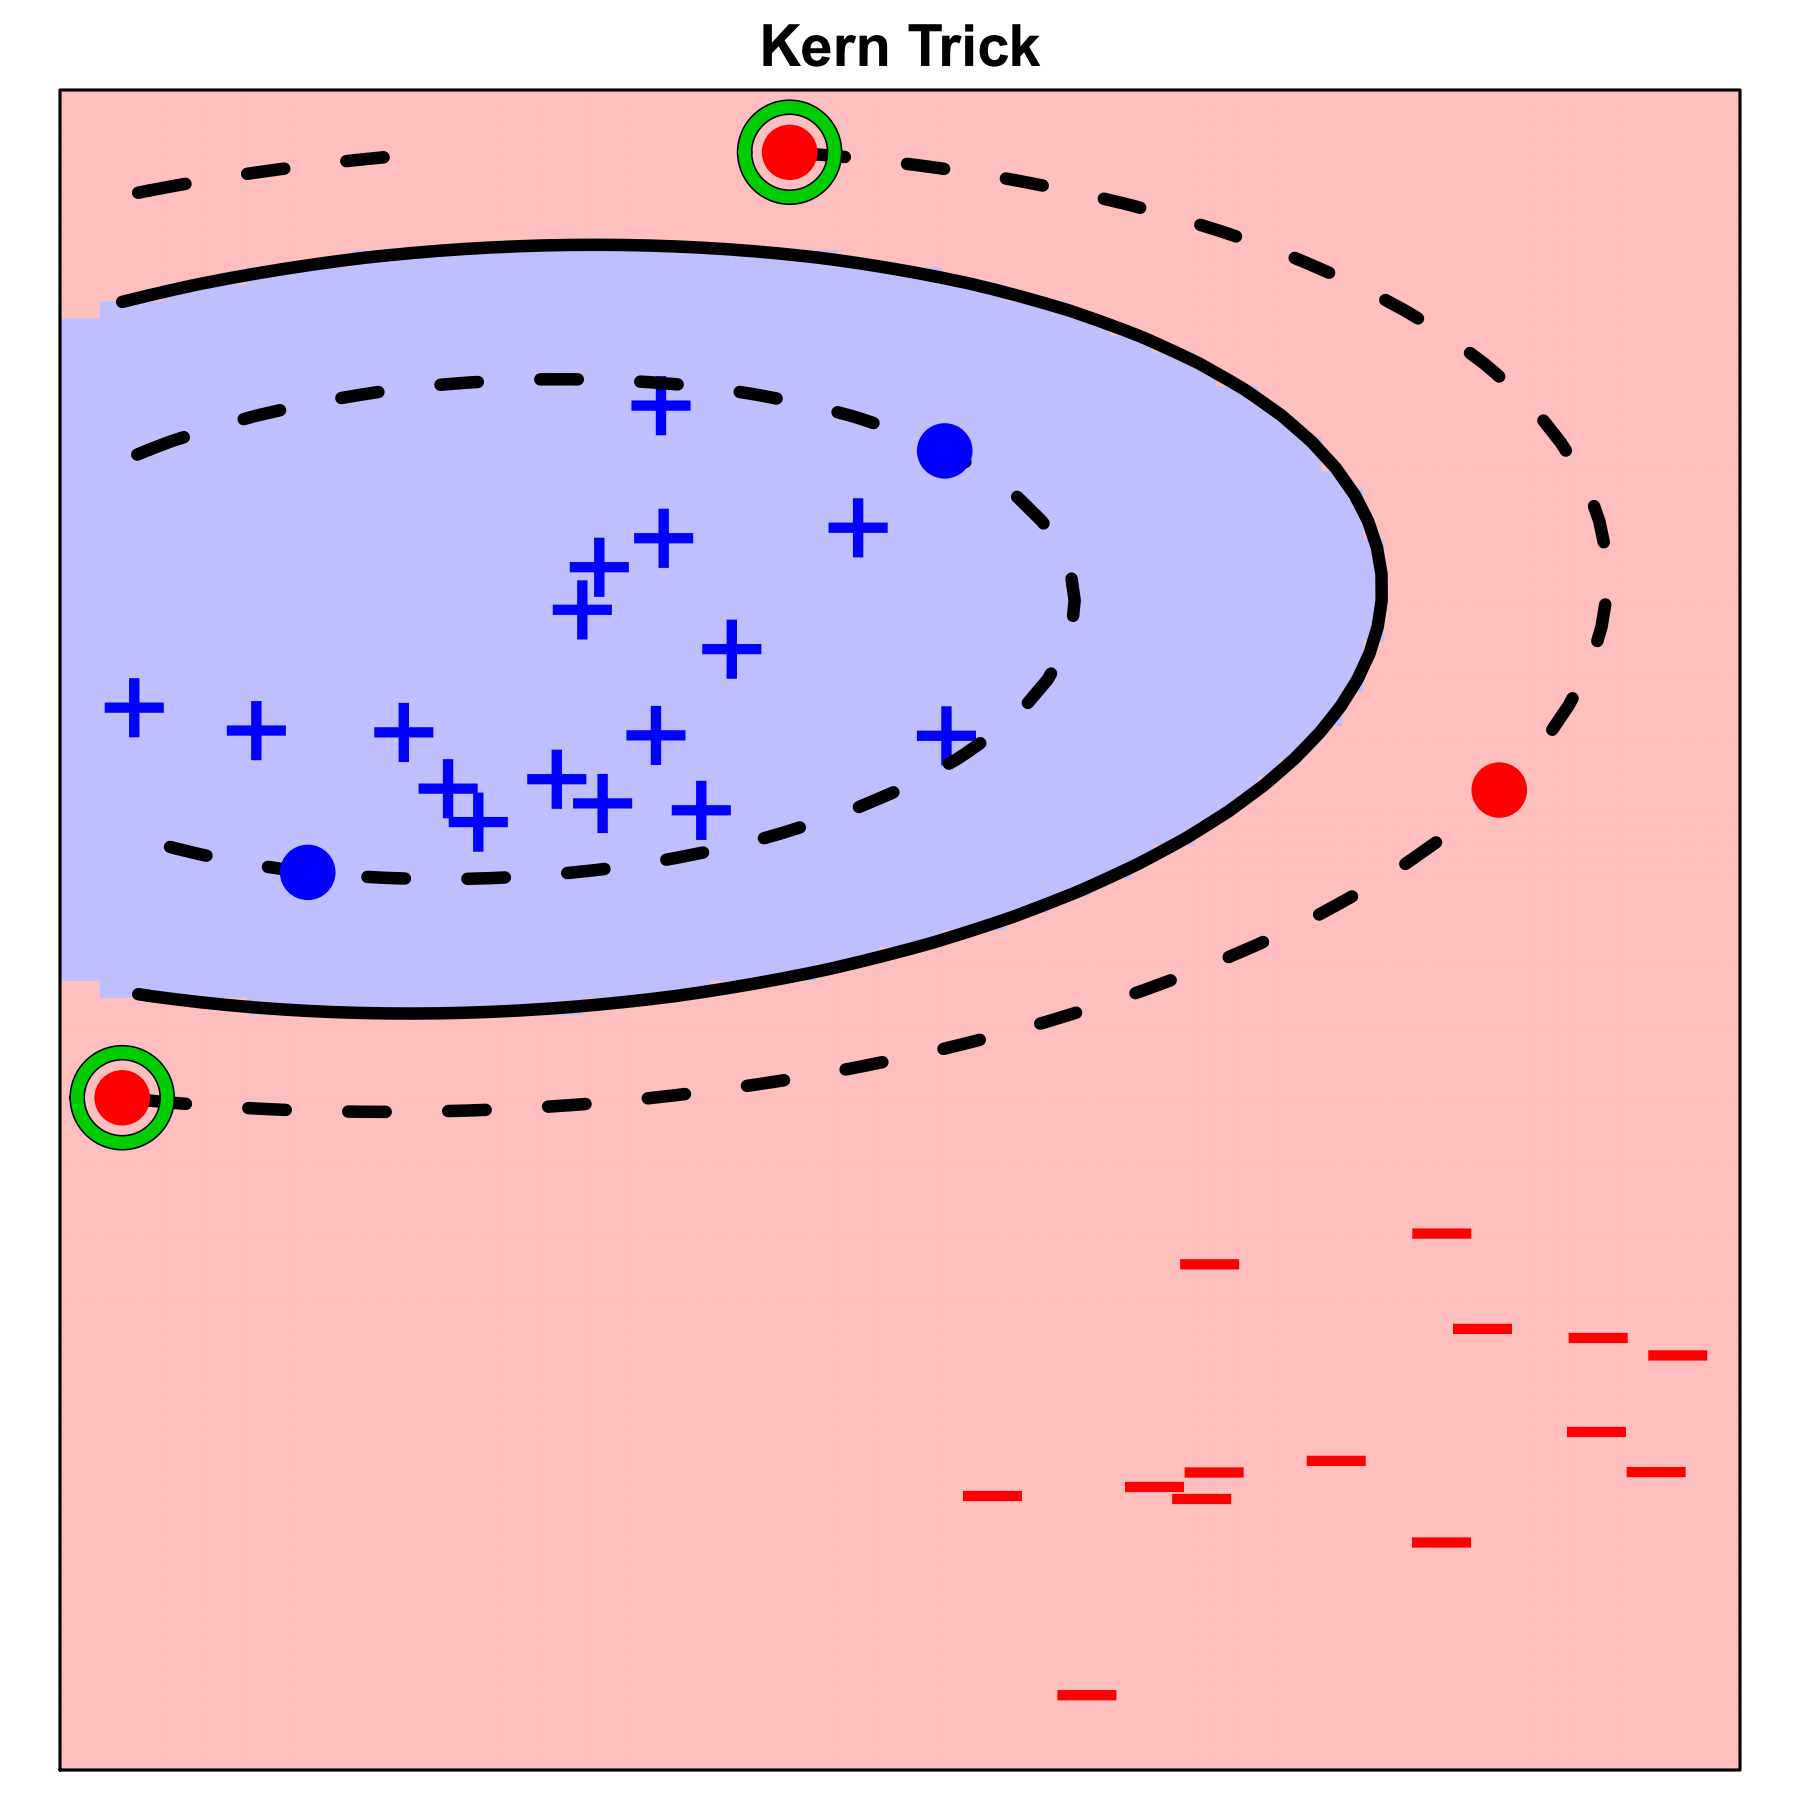
\includegraphics[width=\textwidth]{kerntrick}
\caption{Overfitting beim Kern Trick}
\label{fig:kerntrick}
\end{minipage}
\hspace{0.1cm}
\begin{minipage}[b]{0.5\linewidth}
\centering
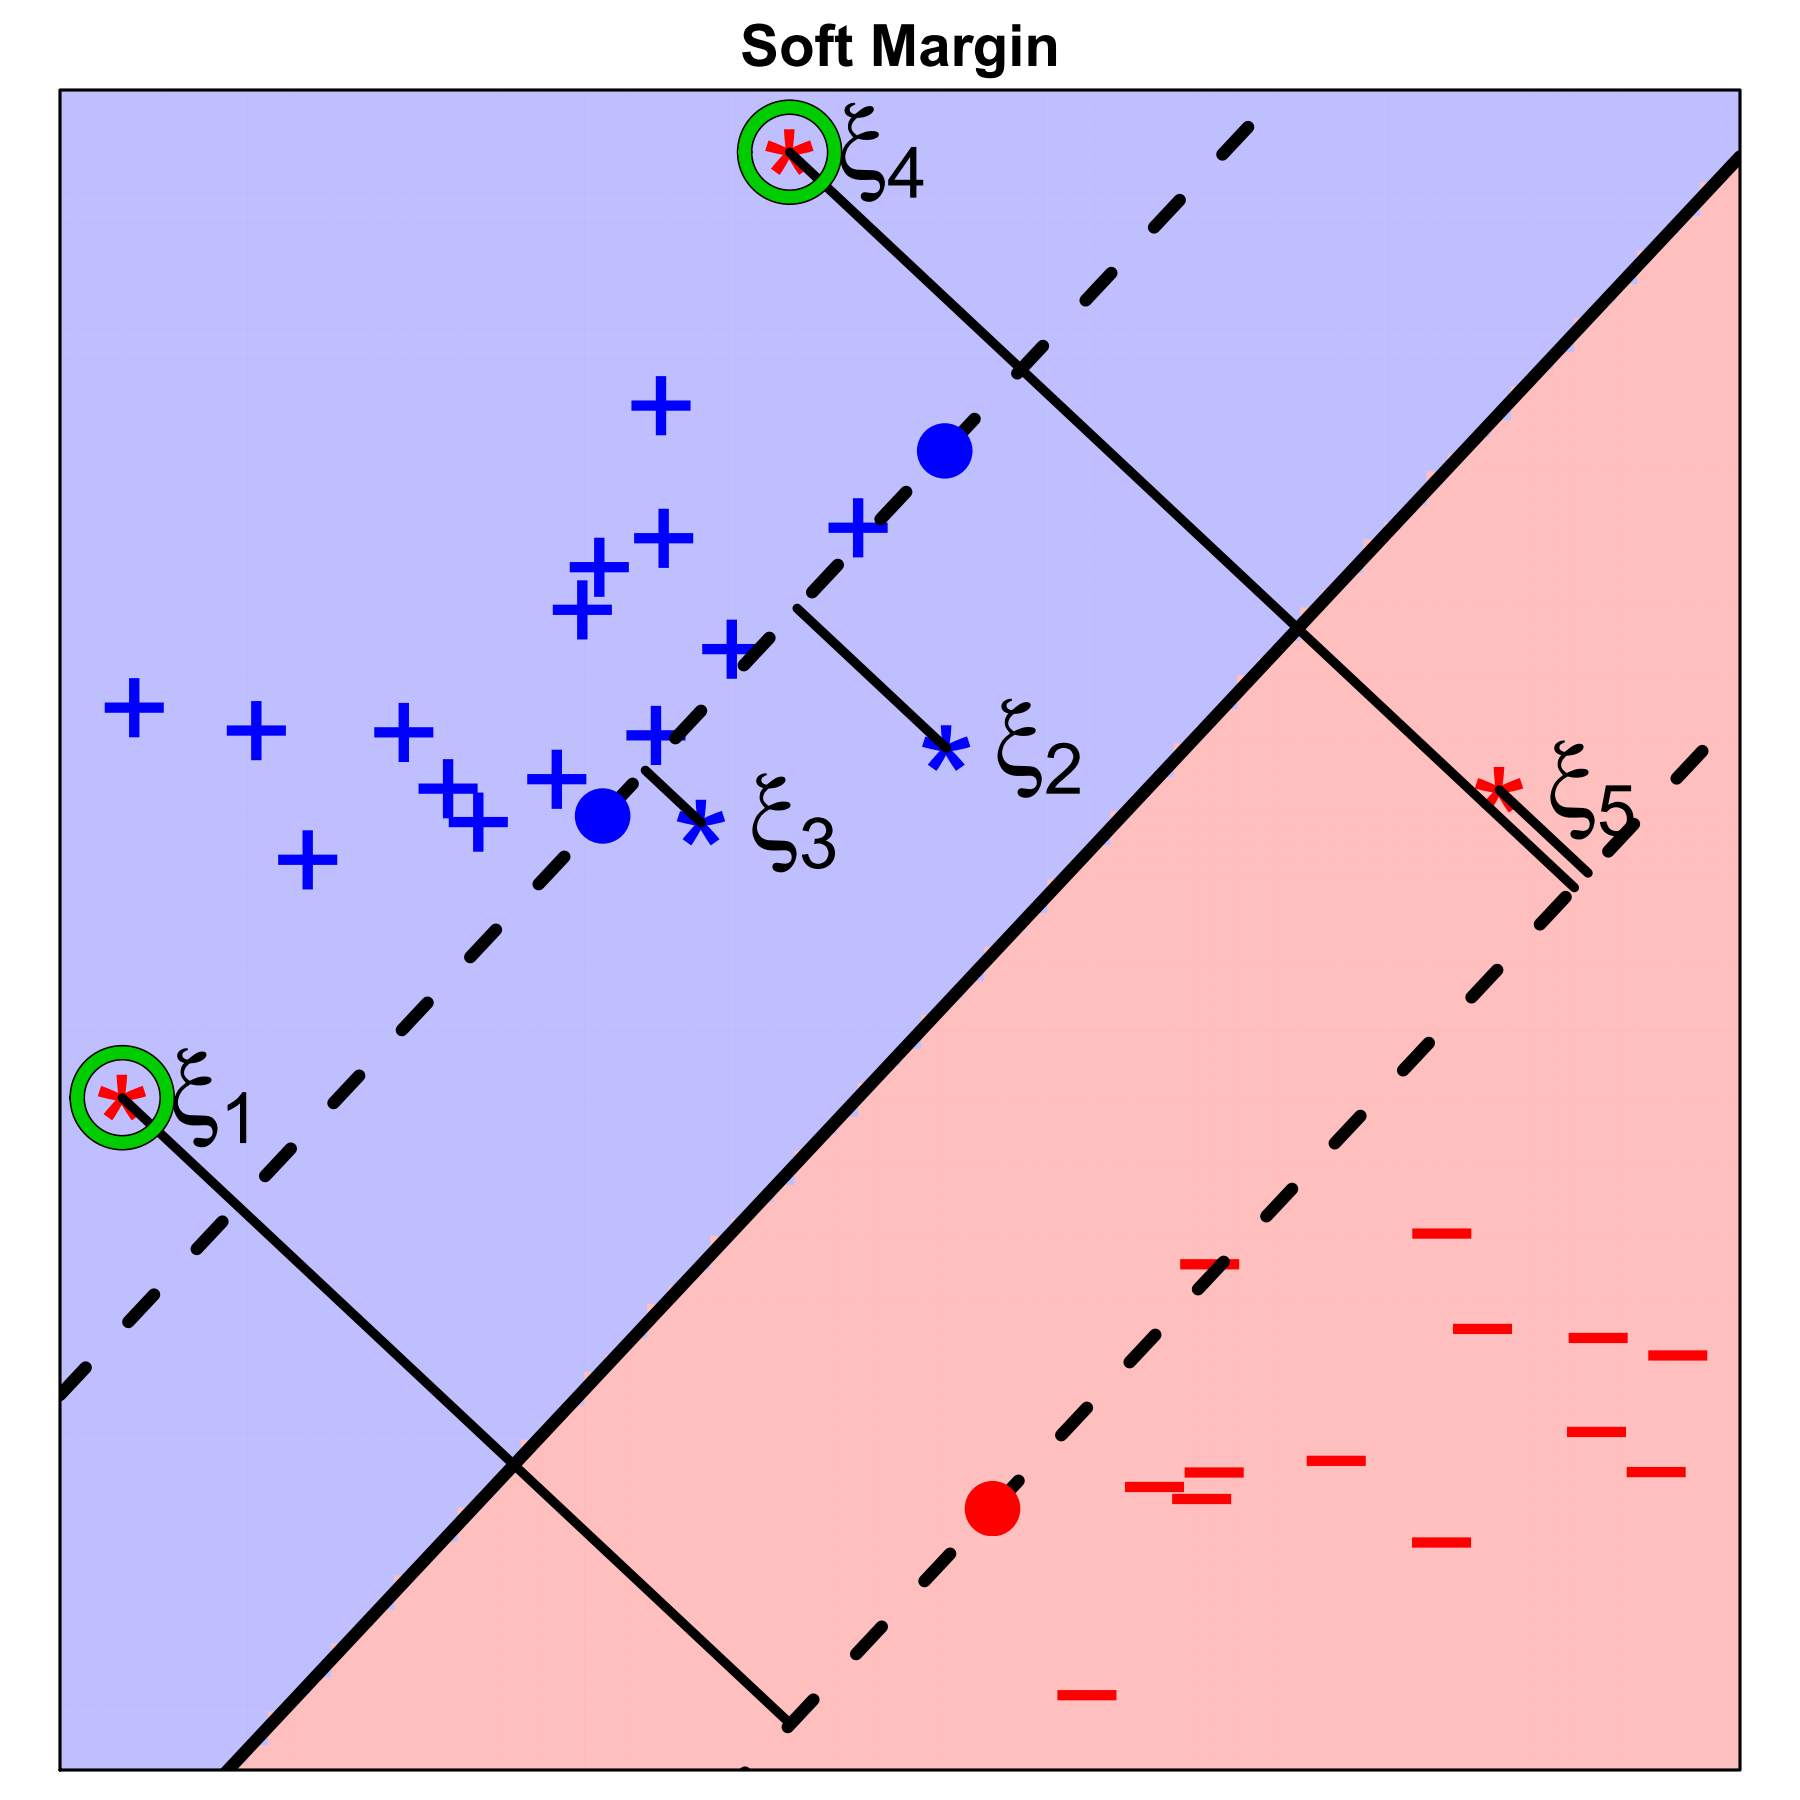
\includegraphics[width=\textwidth]{softmargin}
\caption{Zulassung von Ausrei�ern}
\label{fig:softmargin}
\end{minipage}
\end{figure}

%Je mehr Fehlklassifizierte Datenpunkte, desto gr��er die Summe $\sum_{i=1}^N \xi_i$. Auch nimmt diese Summe mit der Breite des Randes zu, da 
Je breiter der Rand, desto mehr Beobachtungen liegen innerhalb des Randes oder auf der falschen Seite der Hyperebene. Die Summe der Schlupfvariablen $\sum_{i=1}^N \xi_i$ nimmt damit zu. Man m�chte verhindern, dass diese Summe zu gro� wird. Daher ben�tigt man einen Kompromiss zwischen
dem Maximieren des Randes (bzw. $\min \frac{1}{2} ||\mathbf{w}||^2$) und dem Minimieren von $\sum_{i=1}^N \xi_i$. Das Optimierungsproblem aus Kapitel \ref{Optimierungsproblem} wird umformuliert zu
\begin{equation*}
\label{eq:softmargin}
\begin{aligned}
& \min_{\mathbf{w},b, \pmb{\xi}}
& &\frac{1}{2} ||\mathbf{w}||^2 + C \sum_{i=1}^N \xi_i \\
& \text{NB:}
& & y_i (\mathbf{w}^\top \mathbf{x}_i + b) \geq 1 - \xi_i, \\
&&& \xi_i \geq 0, \hspace{8pt} \forall i = 1, \hdots, N.
%&&& \forall i = 1, \hdots, N.
\end{aligned}
\end{equation*}
Der Parameter $C$ kann durch Kreuzvalidierung bestimmt werden und steuert wie stark die Summe $\sum_{i=1}^N \xi_i$ bestraft wird:

\begin{itemize}
\item bei gro�em $C$: \\ Minimierung von $\sum_{i=1}^N \xi_i$ ist wichtiger $\rightarrow$ weniger Schlupfvariablen $\rightarrow$ kleiner Rand
\item bei kleinem $C$: \\ Maximierung des Randes ist wichtiger $\rightarrow$ mehr Schlupfvariablen $\rightarrow$  $\sum_{i=1}^N \xi_i$ gr��er
%\item $C \rightarrow \infty$:
%\item $C \rightarrow 0$:
\end{itemize}

%\newpage

Die dazugeh�rige Lagrange-Funktion 

$$\hspace{-10pt}L(\mathbf{w},b,\pmb{\xi},\pmb{\alpha},\pmb{\mu}) =  \frac{1}{2} ||\mathbf{w}||^2 + C \sum_{i=1}^N \xi_i - \sum_{i=1}^{N} \alpha_i  (y_i (\mathbf{w}^\top \mathbf{x}_i + b) - (1- \xi_i)) - \sum_{i=1}^N \mu_i \xi_i $$

mit Lagrange-Multiplikatoren $\alpha_i \geq 0$ und $\mu_i \geq 0$ wird bez�glich der Prim�rvariablen $\mathbf{w},b \text{ und } \pmb{\xi}$ minimiert und bez�glich $\pmb{\alpha}$ maximiert. Es ergeben sich dieselben L�sungen wie in Gleichung (\ref{primal1}) - (\ref{primal2}) und die zur Minimierung bez�glich $\pmb{\xi}$ hinzukommende L�sung
\begin{align}
\label{primal3}
\frac{\partial L(\mathbf{w},b,\pmb{\xi},\pmb{\alpha},\pmb{\mu})}{\partial \pmb{\xi}} = 0          & \Rightarrow C = \alpha_i + \mu_i \hspace{8pt} \forall i=1,\hdots, N.
\end{align}
Als Lagrange-duale Funktion folgt
\begin{align*}
W(\pmb{\alpha}) &=\min_{\mathbf{w}, b, \pmb{\xi}} L(\mathbf{w},b,\pmb{\xi},\pmb{\alpha},\pmb{\mu})\\
&=\min_{\mathbf{w}, b, \pmb{\xi}} \left ( \frac{1}{2} \mathbf{w}^\top \mathbf{w} \; + C \sum_{i=1}^N \xi_i - \sum_{i=1}^N \alpha_i (y_i (\mathbf{w}^\top \mathbf{x}_i +b) - (1 - \xi_i)) - \sum_{i=1}^N \mu_i \xi_i \right )\\
&=\min_{\mathbf{w}, b, \pmb{\xi}} \left ( \frac{1}{2} \mathbf{w}^\top \mathbf{w} \; + \sum_{i=1}^N C \xi_i - \sum_{i=1}^N  \alpha_i y_i \mathbf{w}^\top \mathbf{x}_i 
- \sum_{i=1}^N \alpha_i y_i b + \sum_{i=1}^N \alpha_i - \sum_{i=1}^N \alpha_i \xi_i  - \sum_{i=1}^N \mu_i \xi_i \right )\\
&\stackrel{(\ref{primal3})}= \min_{\mathbf{w}, b} \left ( \frac{1}{2} \mathbf{w}^\top \mathbf{w} \; \cancel{+ \sum_{i=1}^N (\alpha_i + \mu_i ) \xi_i} 
- \sum_{i=1}^N  \alpha_i y_i \mathbf{w}^\top \mathbf{x}_i 
- b \sum_{i=1}^N \alpha_i y_i  + \sum_{i=1}^N \alpha_i \cancel{- \sum_{i=1}^N (\alpha_i + \mu_i) \xi_i} \right )\\
&\stackrel{(\ref{primal1})}= \min_{\mathbf{w}} \left ( \frac{1}{2} \mathbf{w}^\top \mathbf{w} \; - \sum_{i=1}^N  \alpha_i y_i \mathbf{w}^\top \mathbf{x}_i + \sum_{i=1}^N \alpha_i \right )\\
&\stackrel{(\ref{primal2})}= \frac{1}{2} \sum_{i=1}^N \alpha_i y_i \mathbf{x}_i^\top \sum_{j=1}^N \alpha_j y_j \mathbf{x}_j - \sum_{i=1}^N \alpha_i y_i \left ( \sum_{j=1}^N \alpha_j y_j \mathbf{x}_j^\top \right ) \mathbf{x}_i + \sum_{i=1}^N \alpha_i \\
&=\frac{1}{2} \sum_{i,j=1}^N \alpha_i \alpha_j y_i y_j \mathbf{x}_i^{\top} \mathbf{x}_j - \sum_{i,j=1}^N \alpha_i \alpha_j y_i y_j \mathbf{x}_i^{\top} \mathbf{x}_j + \sum_{i=1}^N \alpha_i \\
&= -\frac{1}{2} \sum_{i,j=1}^N \alpha_i \alpha_j y_i y_j \mathbf{x}_i^{\top} \mathbf{x}_j + \sum_{i=1}^N \alpha_i.
\end{align*}
Hier ist die Lagrange-duale Funktion identisch zum Fall linear trennbarer Daten (vgl. Kapitel \ref{Optimierungsproblem}). Das duale Optimierungsproblem 
\begin{gather*}
\label{primalsoft}
%\begin{aligned}
\max_{\pmb{\alpha}}  W(\pmb{\alpha})
= \max_{\pmb{\alpha}} \left ( \sum_{i=1}^N \alpha_i - \frac{1}{2} \sum_{i,j=1}^N \alpha_i \alpha_j y_i y_j \mathbf{x}_i^{\top} \mathbf{x}_j \right )\\
\text{NB:} \hspace{20pt} 0 \leq \alpha_i \leq C, \hspace{20pt} \sum_{i=1}^N \alpha_i y_i = 0 \hspace{20pt} \forall i= 1, \hdots, N
%\end{aligned}
\end{gather*}
hat im Vergleich zu Gleichung (\ref{dual}) die zus�tzliche Nebenbedingung $\alpha_i \leq C$, die sich aus Gleichung (\ref{primal3}) herleiten l�sst: $C = \alpha_i + \mu_i \; \Leftrightarrow \; \alpha_i = C - \mu_i \;  \stackrel{\mu_i \geq 0} \Longrightarrow \;  \alpha_i \leq C$ (\citealp[vgl.][Kap. 4.2]{ben2010user}; \citealp[Kap. 2.2]{gunn1998support}). 

Das weitere Vorgehen zur Bestimmung der Hyperebenenparameter $(\mathbf{w},b)$ ist analog zum linear trennbaren Fall.

\chapter{Anwendungsbeispiel}

Das folgende Beispiel ist mit der statistischen Software \texttt{R} (\citealp{R}) und dem Zusatzpaket \texttt{svmpath} (\citealp{svmpath}) erstellt worden. Der dazugeh�rige R-Code befindet sich in der mitgelieferten Datei \texttt{Anwendungsbeispiel.R}. Eine weitere Umsetzung f�r Support Vector Machines in \texttt{R} ist unter anderem in der Funktion 
%\texttt{ksvm()} aus dem Paket \texttt{kernlab} \citep{kernlab} oder in der Funktion 
\texttt{svm()} aus dem Paket \texttt{e1071} (\citealp{e1071}) zu finden.

Zun�chst werden $200$ Beobachtungen simuliert, die dann durch zuf�lliges Ziehen im Verh�ltnis von $4:1$ in Trainingsdaten und Testdaten aufgeteilt werden. 
Die $N=160$ Trainingsdaten in Abbildung \ref{train} sollen das Zwei-Spiralen-Problem in einem zweidimensionalen Variablenraum nachstellen. Dabei handelt es sich um ein bekanntes bin�res Klassifikationsproblem, bei dem die zwei Klassen spiralf�rmig miteinander verzahnt sind.

\begin{figure}[h]
\centering
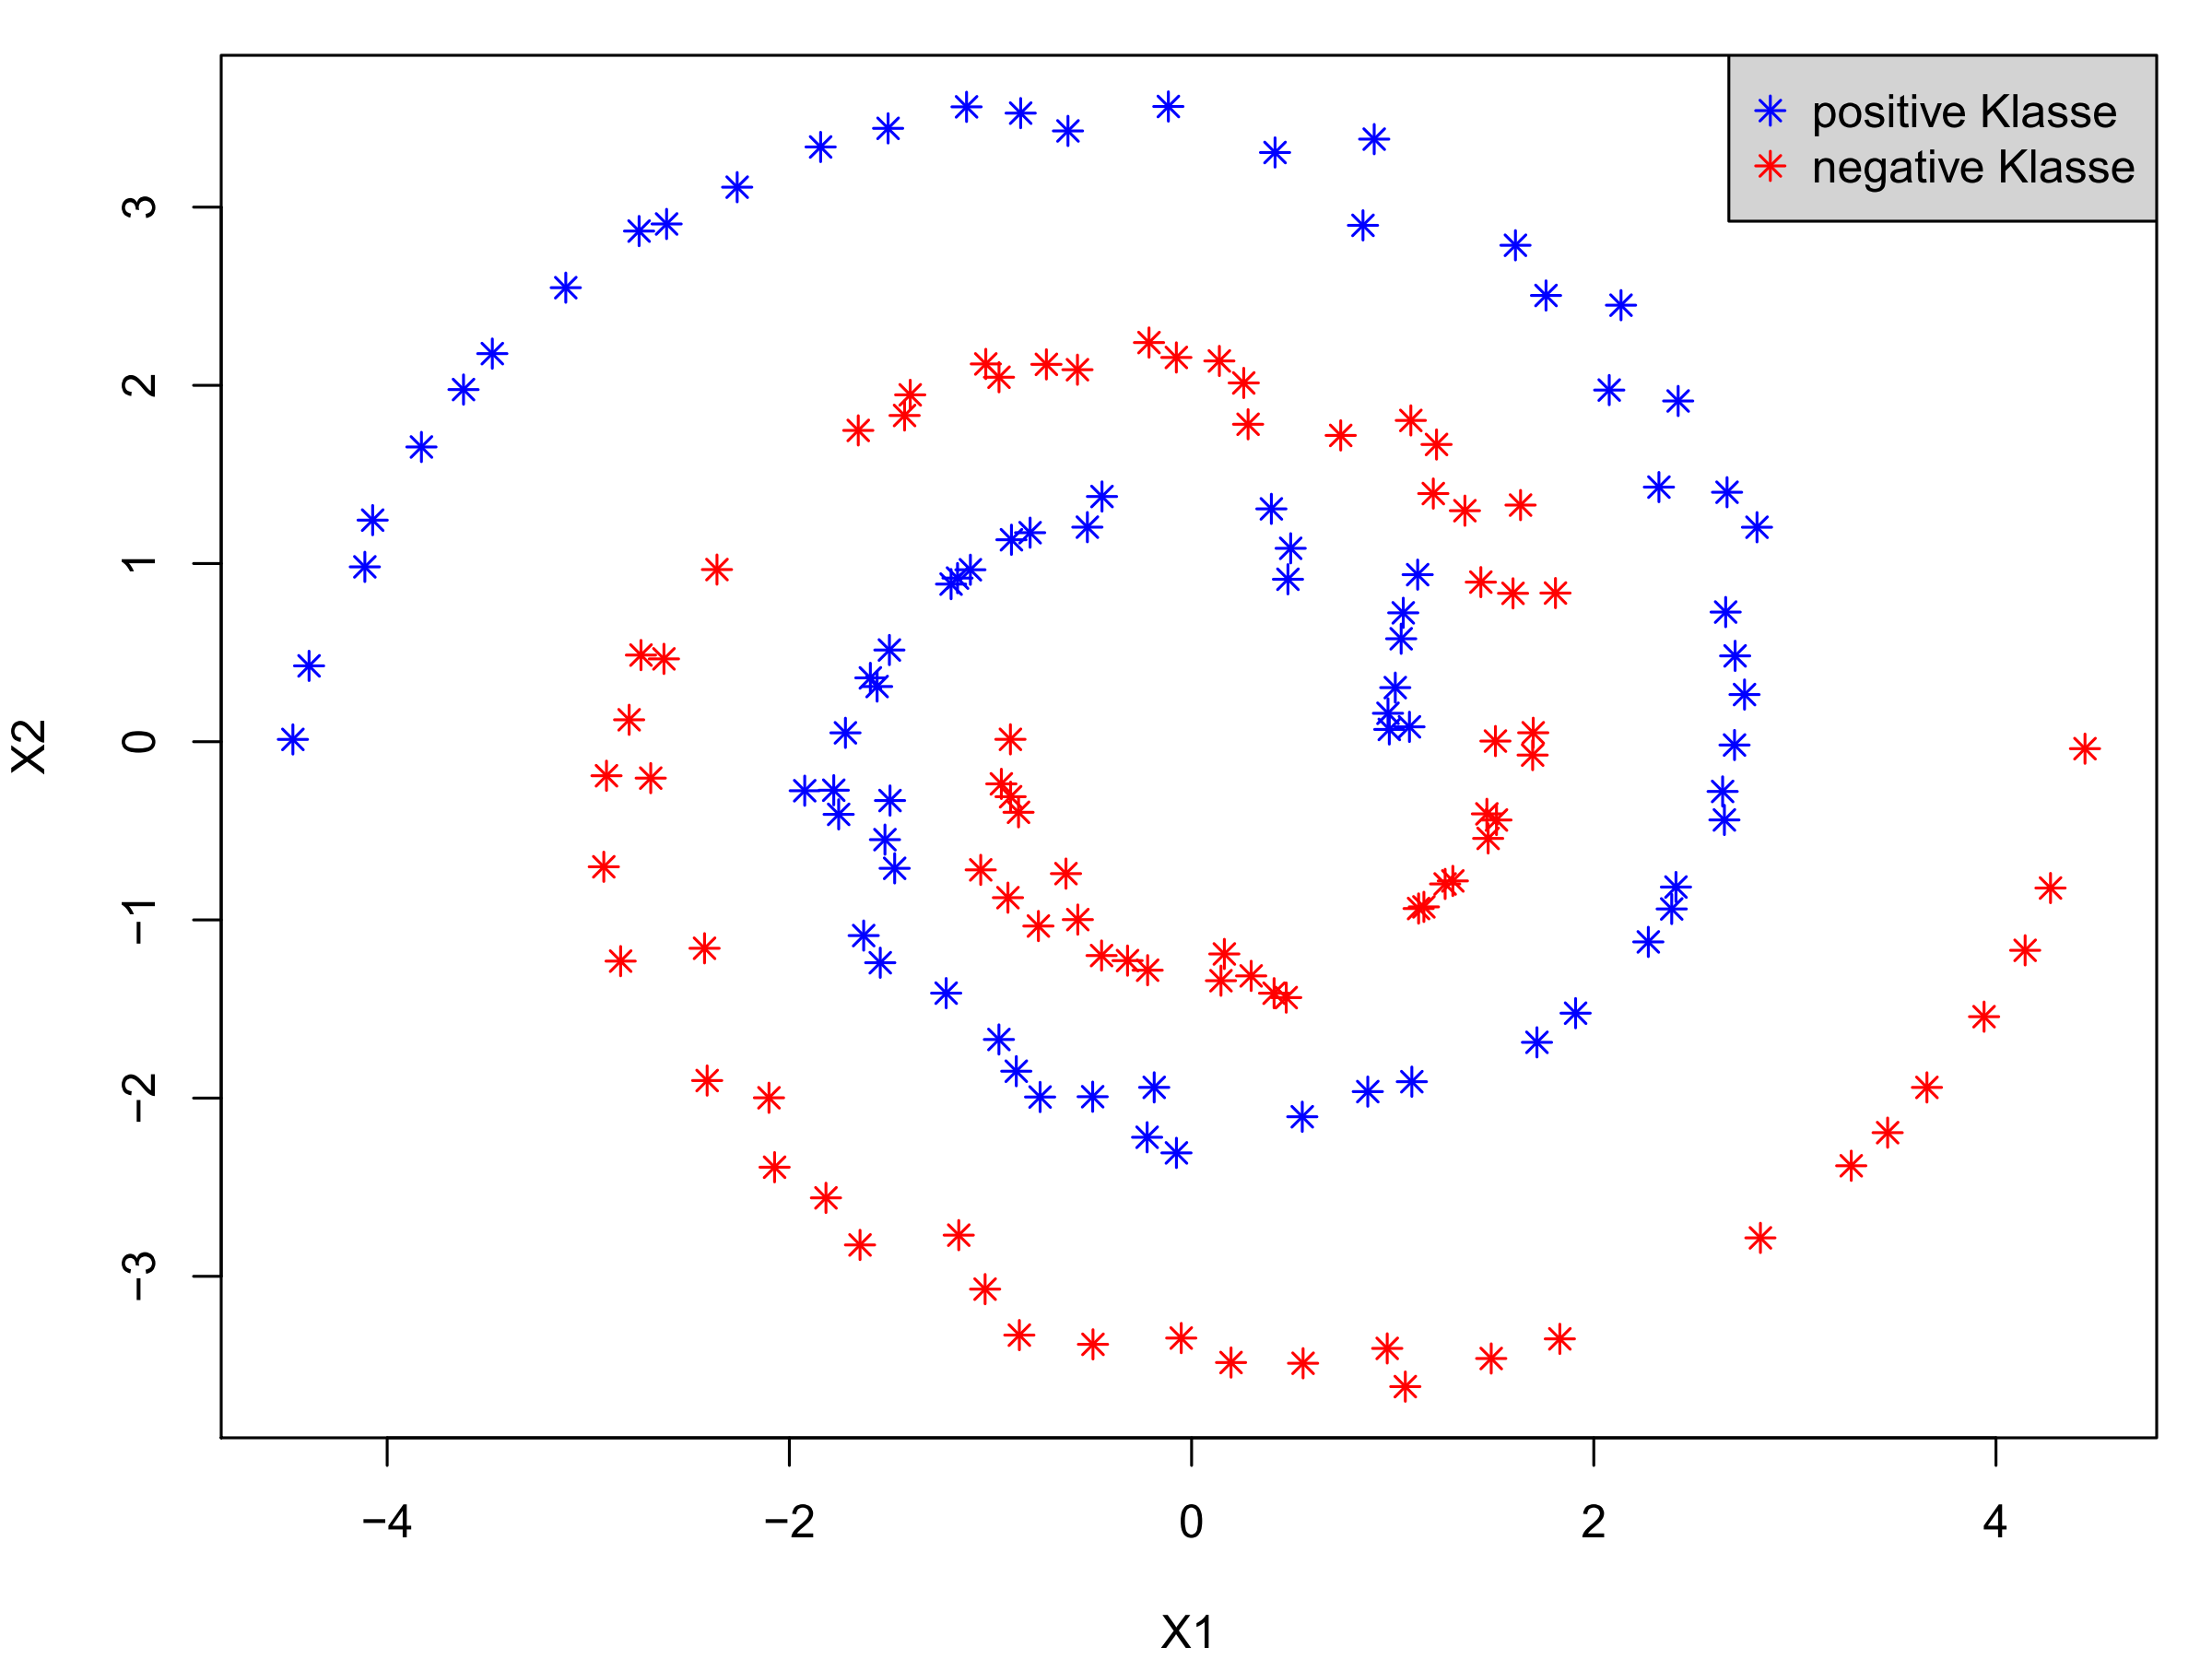
\includegraphics[width=\textwidth]{traintest_01.png}
\caption{Spiralf�rmige Trainingsdaten}
\label{train}
\end{figure}

Gesucht ist eine Hyperebene, welche die Trainingsdaten f�r m�glichst viele Beobachtungen voneinander trennt. Die Testdaten sollen anschlie�end, durch die auf Basis der Trainingsdaten gesch�tzten Hyperebene, m�glichst fehlerfrei in die beiden Klassen zugeordnet werden.

In Abbildung \ref{polyKern} wurde die Hyperebene durch Verwendung einer polynomialen Kernfunktion zweiten Grades der Form $K(\mathbf{x}_i,\mathbf{x}_j) = (\mathbf{x}_i^\top \mathbf{x}_j + 1)^2$ ermittelt. Im Vergleich dazu wurde in Abbildung \ref{rbfKern} als Kernfunktion eine gau�sche radiale Basisfunktion (RBF) der Form $K(\mathbf{x}_i,\mathbf{x}_j) = \exp(-||\mathbf{x}_i-\mathbf{x}_j||)$ verwendet.

\begin{figure}[h]
\begin{minipage}[b]{0.5\linewidth}
\centering
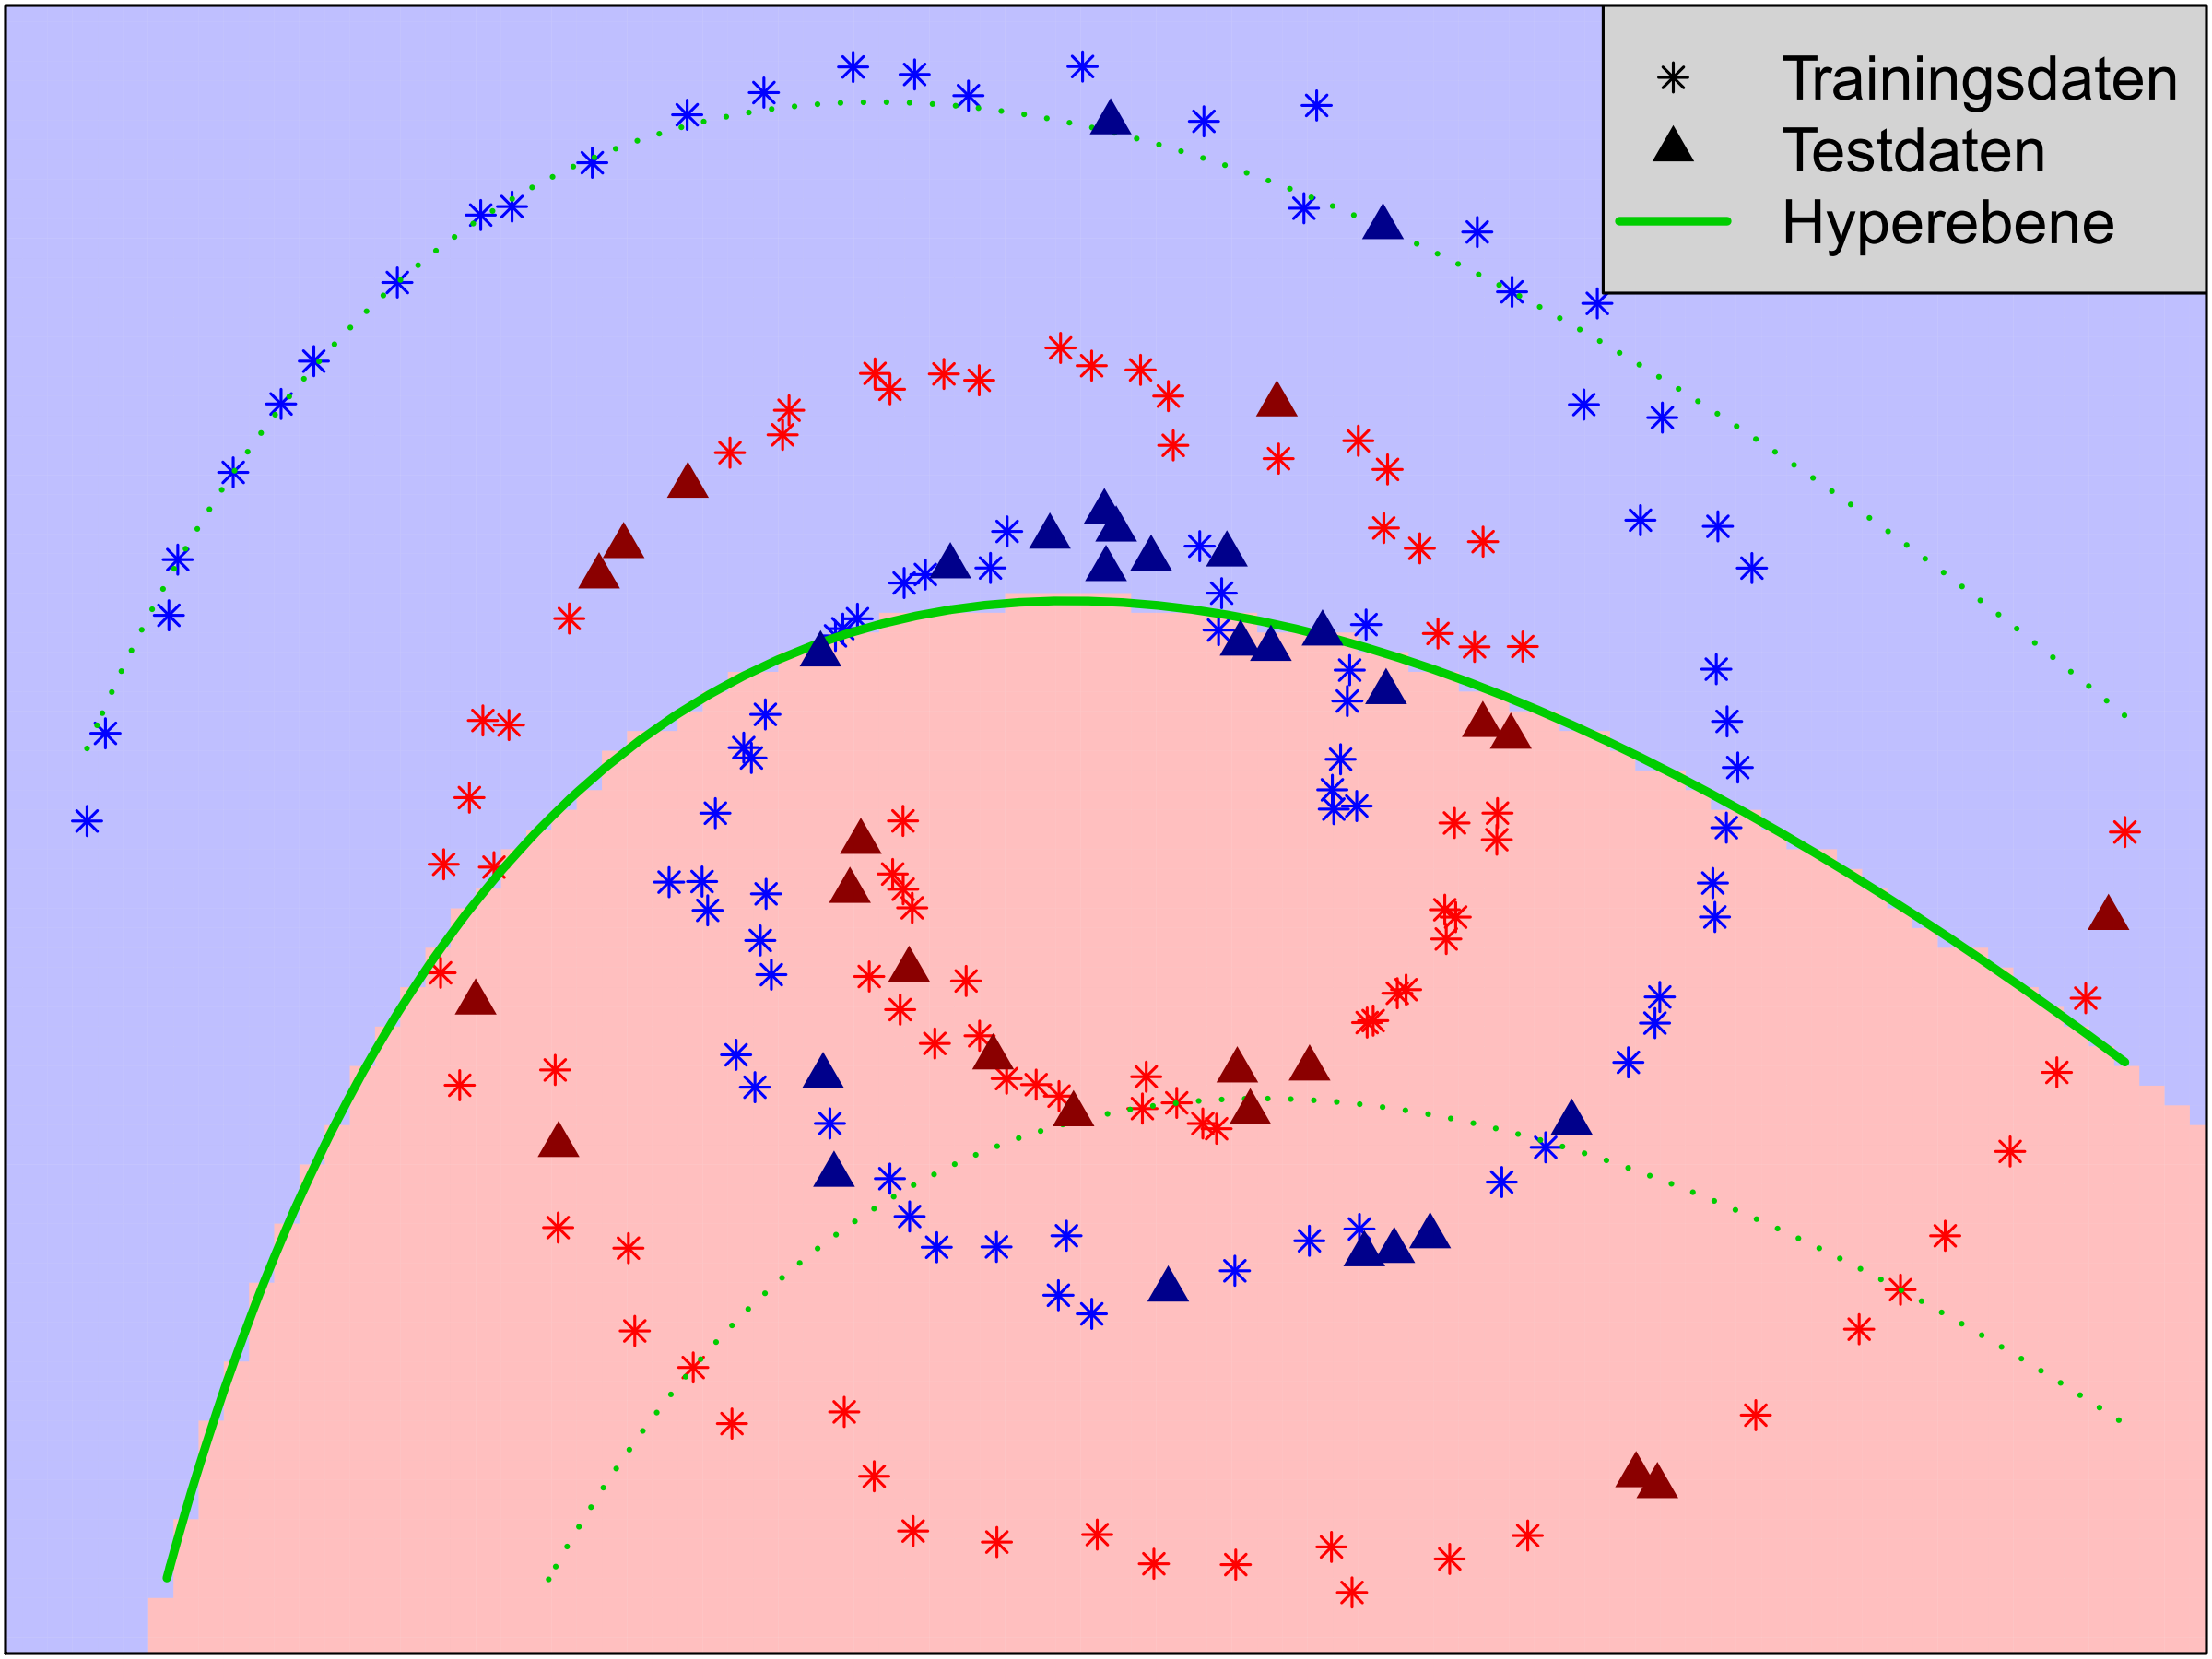
\includegraphics[width=\textwidth]{traintest_03.png}
\caption{polynomiale Kernfunktion}
\label{polyKern}
\end{minipage}
\hspace{0.1cm}
\begin{minipage}[b]{0.5\linewidth}
\centering
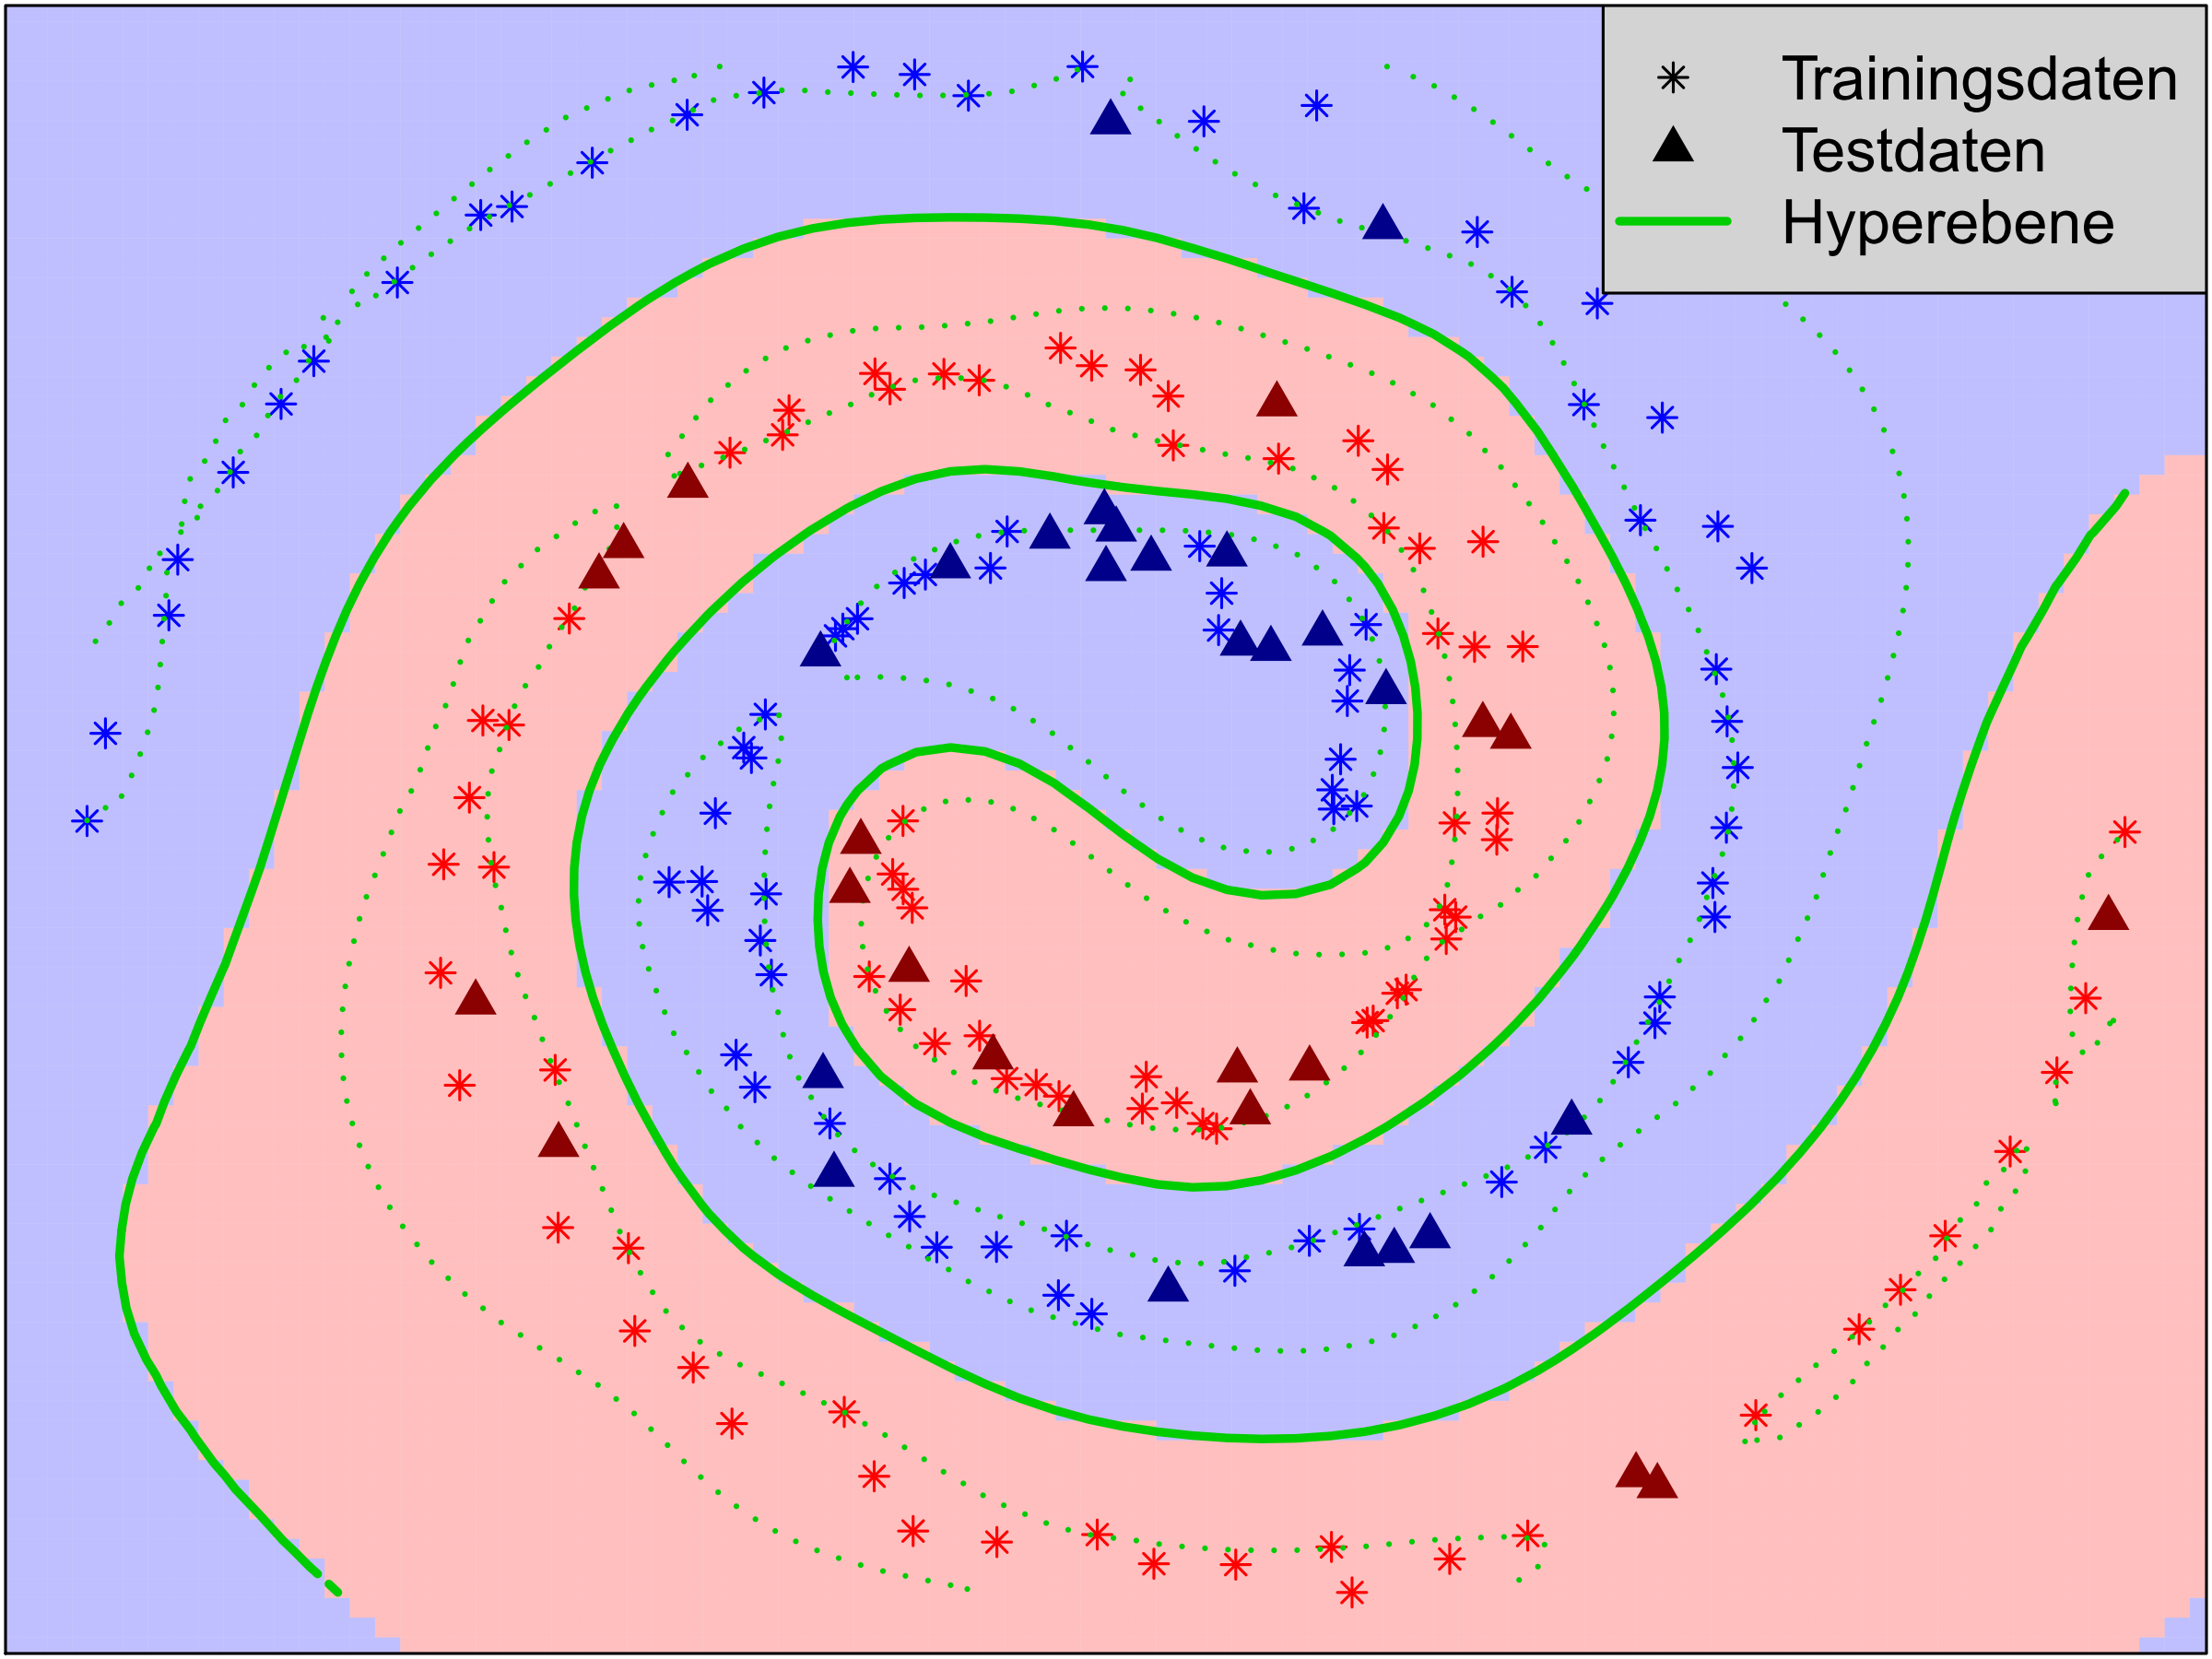
\includegraphics[width=\textwidth]{traintest_02.png}
\caption{gau�sche RBF}
\label{rbfKern}
\end{minipage}
\end{figure}

%\begin{figure}[h]
%\centering
%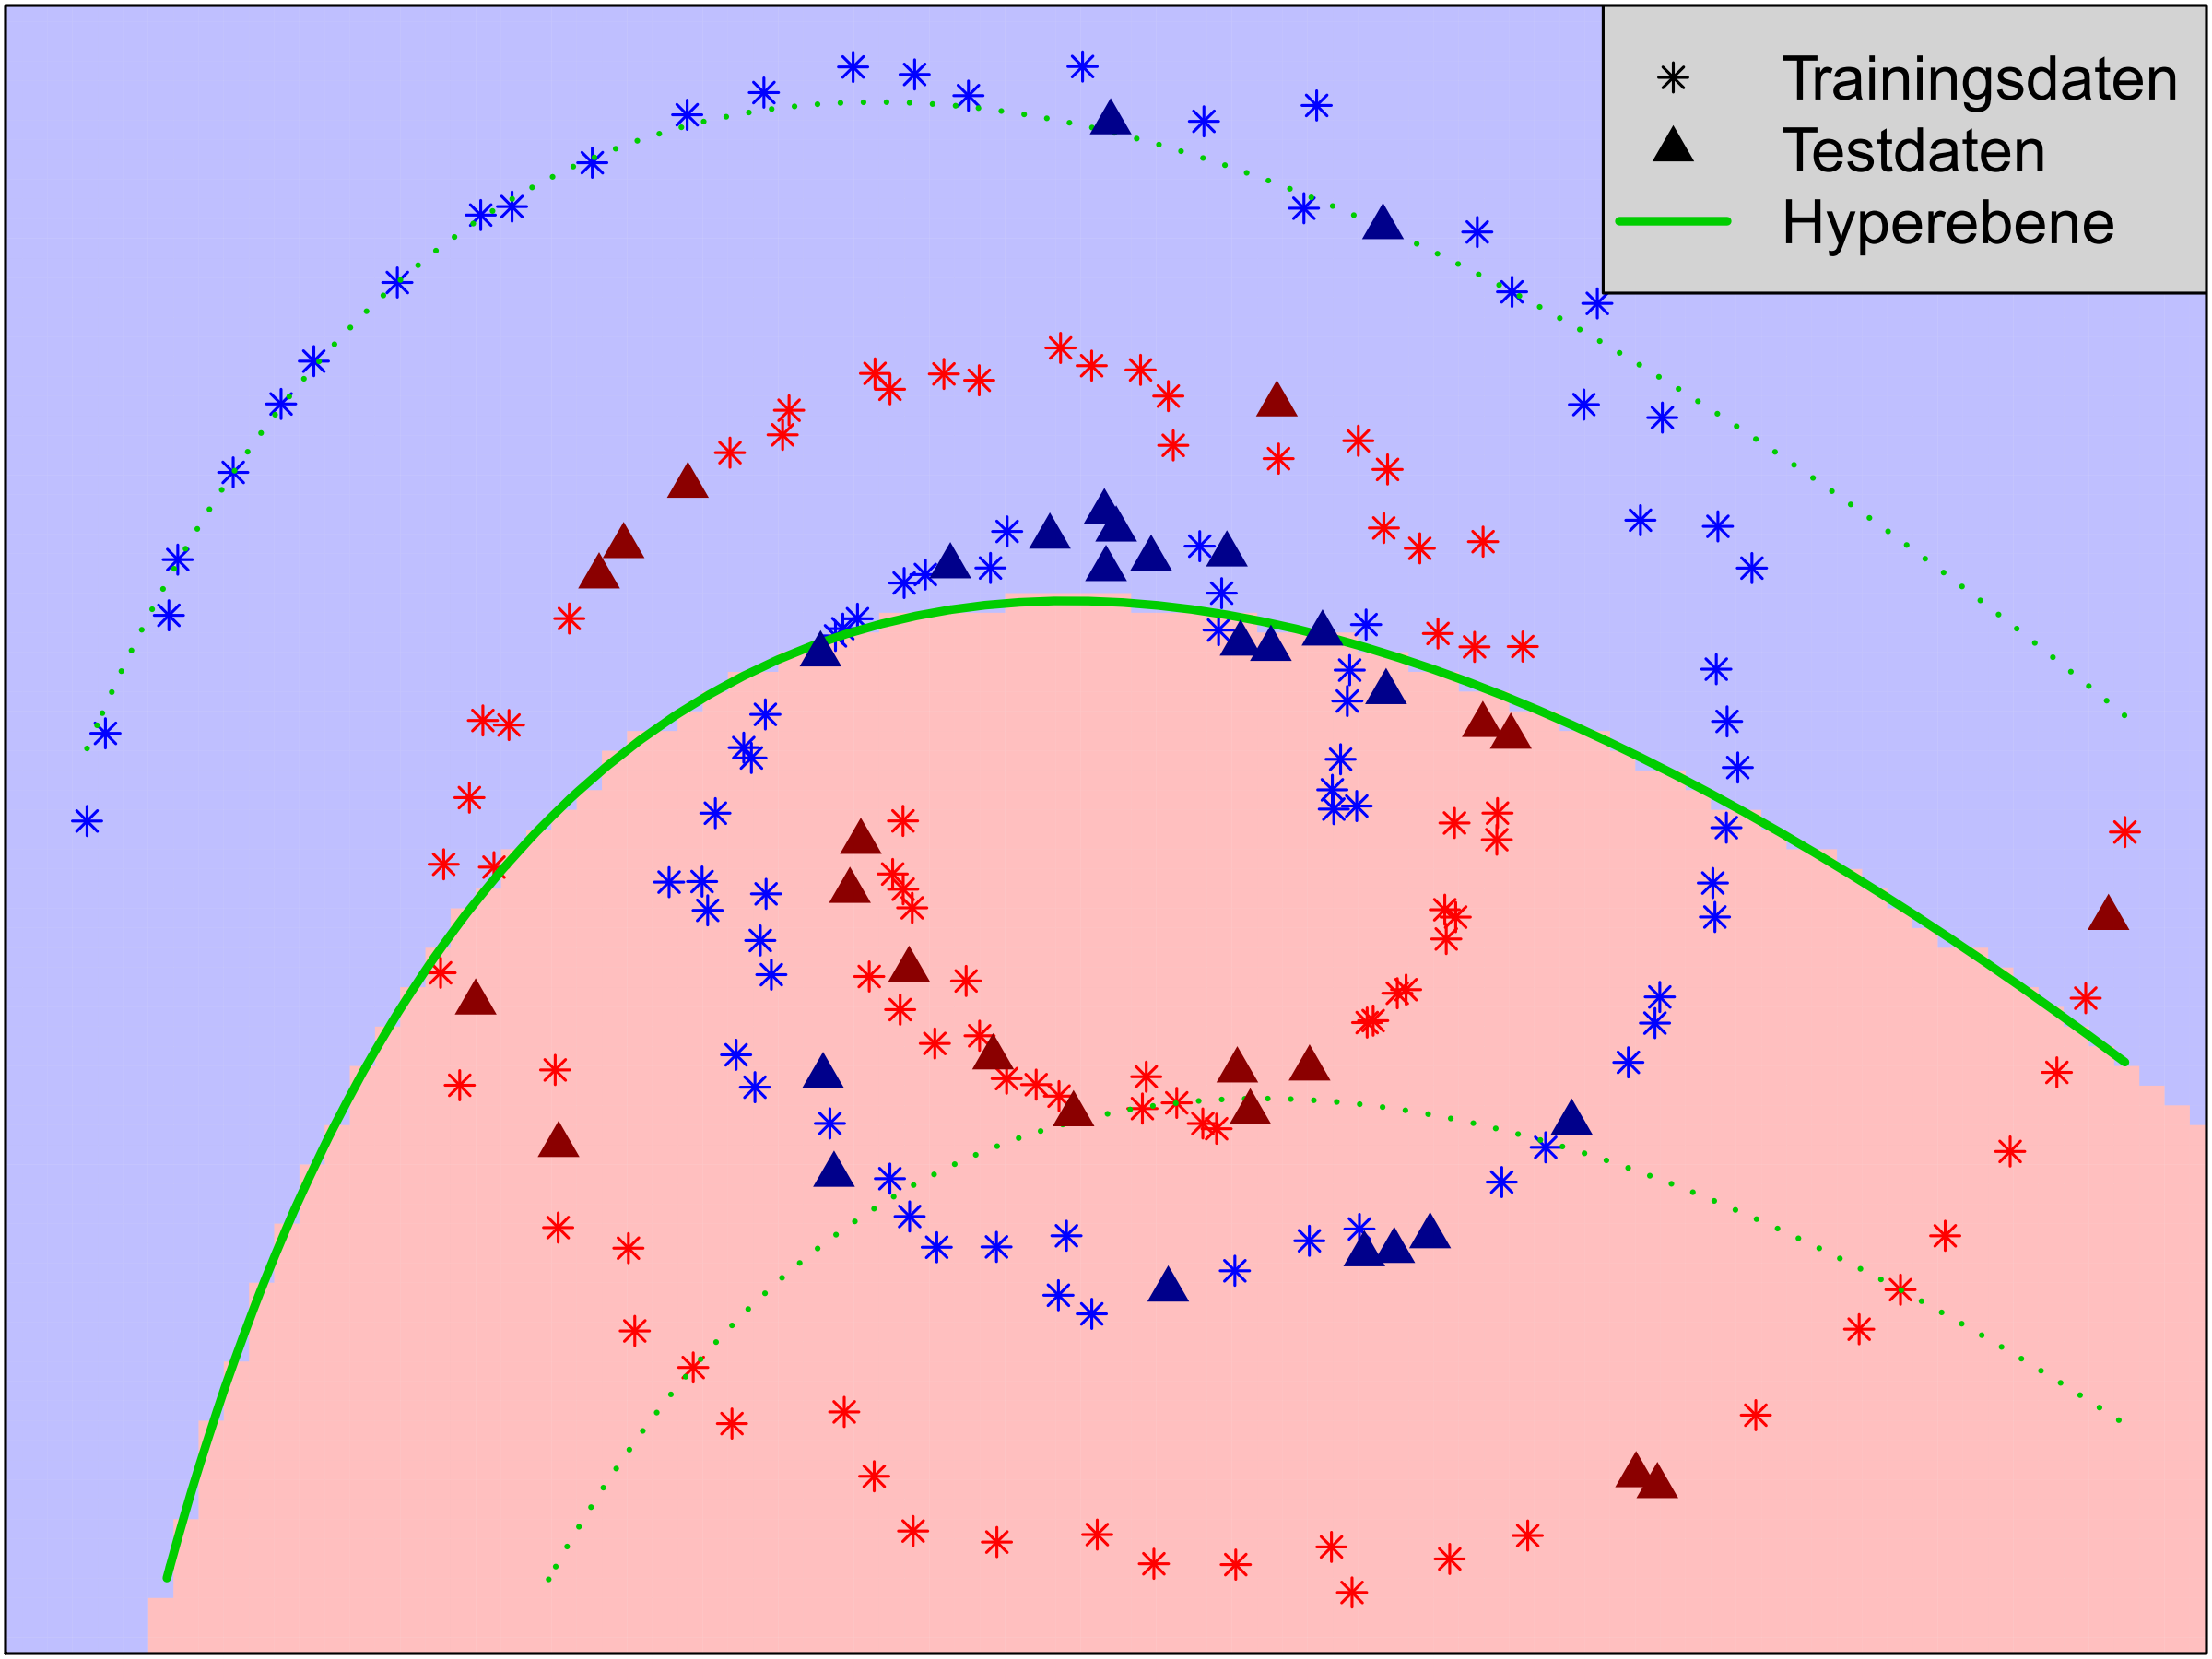
\includegraphics[width=0.6\textwidth]{traintest_03.png}
%\caption{polynomiale Kernfunktion}
%\label{polyKern}
%\end{figure}
%\begin{figure}[h]
%\centering
%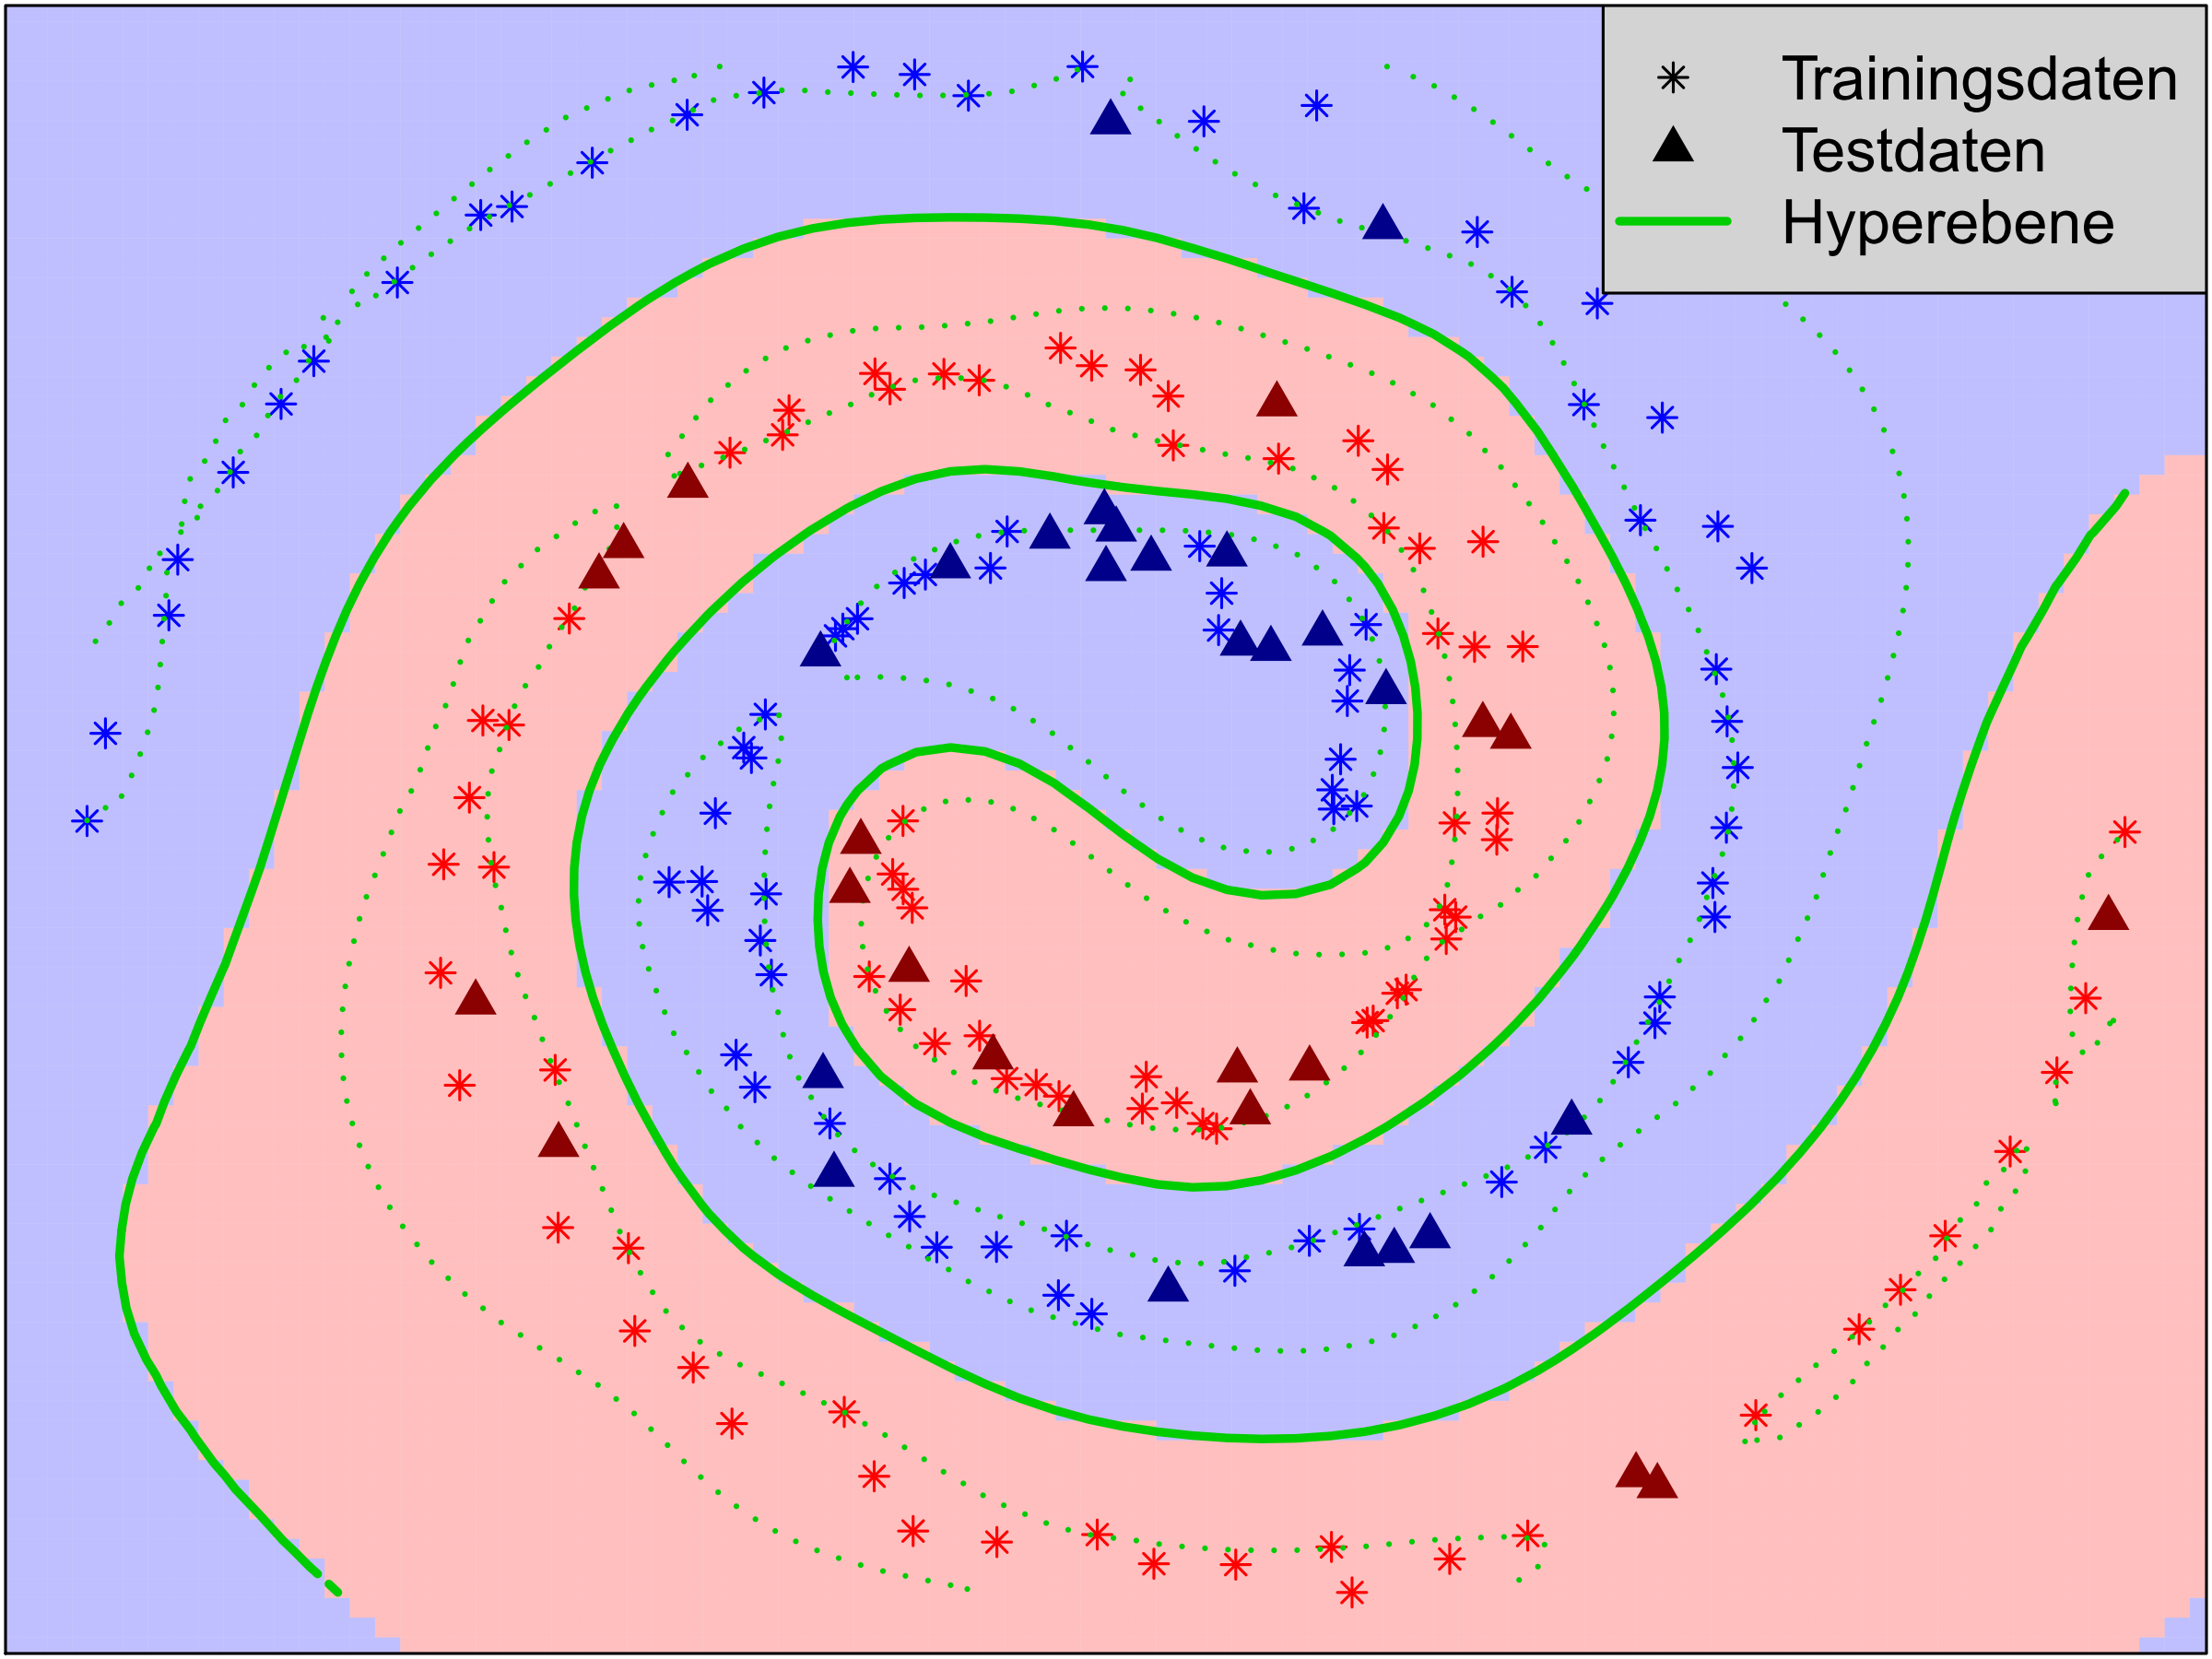
\includegraphics[width=0.6\textwidth]{traintest_02.png}
%\caption{gau�sche RBF}
%\label{rbfKern}
%\end{figure}

%Hier sieht man dass die polynomiale Kernfunktion wieder einer Ellipse entspricht Wie in Kapitel \ref{sec:kerneltrick} erl�ute
Die polynomiale Kernfunktion kann die spiralf�rmig verzahnten Trainingsdaten hier nicht vollst�ndig voneinander trennen, da die resultierenden Hyperebenen die Form eines Kegelschnitts haben (vgl. Kapitel \ref{sec:kerneltrick}). Die gau�sche radiale Basisfunktion hingegen �berf�hrt den Variablenraum in einen hochdimensionalen Variablenraum, bei dem eine Hyperebene gefunden werden kann, welches die Trainingsdaten vollst�ndig voneinander trennt. 
Tabelle \ref{tab:missclass} zeigt dabei die Anzahl bzw. den Anteil der fehlklassifizierten Trainingsdaten und Testdaten.

\begin{table}[ht]
\begin{center}
\begin{tabular}{|c||c|c||c|c|}
\hline 
 & \multicolumn{2}{c||}{Trainingsdaten} & \multicolumn{2}{c|}{Testdaten}\\ %\hline
 & Anzahl & Anteil & Anzahl & Anteil \\ 
  \hline
Abbildung \ref{polyKern} & 67 &  41.875 \% &    16 & 40 \% \\ 
   \hline
Abbildung \ref{rbfKern}  & 0 & 0 \% & 0 & 0 \% \\ 
   \hline
\end{tabular}
\end{center}
\caption{Fehlklassifizierungen in Trainingsdaten und Testdaten}
\label{tab:missclass}
\end{table}

%bla \ref{tab:label}
%\begin{table}[t]
%\centering
%\begin{tabular}{c|c}
%4	& 5\\ %table content
%\end{tabular}
%\caption{ba}
%\label{tab:label}
%\end{table}

\chapter{Zusammenfassung und Ausblick}

Wenn das prim�re Optimierungsproblem bekannt ist, lassen sich bei linear trennbaren Daten die Schritte zur Bestimmung der Hyperebenenenparameter $(\mathbf{w}, b)$ wie folgt zusammenfassen:

\begin{enumerate}
\item Lagrangefunktion aufstellen
\item Lagrange-duale Funktion und duales Optimierungsproblem herleiten
\item Lagrange-Multiplikator $\alpha_i$ durch duales Optimierungsproblem bestimmen
\item Richtungsvektor $\mathbf{w} = \sum_{i=1}^N \alpha_i y_i \mathbf{x}_i$ der kanonischen Hyperebene berechnen
\item Verschiebung $b = y_j - \sum_{i=1}^N \alpha_i y_i \mathbf{x}_i^\top \mathbf{x}_j  $ der Hyperebene ermitteln
\item Entscheidungsfunktion 
$f(\mathbf{x}_j) = \text{sgn} \left (\mathbf{w}^\top \mathbf{x}_j + b \right ) =  \text{sgn} \left (\sum_{i=1}^N \alpha_i y_i \mathbf{x}_i^\top \mathbf{x}_j  + b \right )$ aufstellen
\end{enumerate}

Bei nicht linear trennbaren Daten ist eine M�glichkeit die Verwendung des Kern Tricks, der
% mit Hilfe einer Kernfunktion $K$ den Merkmalsvektor $\mathbf{x}$
 die Daten in einem h�herdimensionalen Variablenraum �berf�hrt, in dem sie linear trennbar sind. Die Schritte zur Bestimmung der Hyperebenenenparameter �ndern sich darin, dass der Merkmalsvektor $\mathbf{x}_i$ f�r alle $i=1, \hdots, N$ durch einen h�herdimensionalen Merkmalsvektor $\Phi(\mathbf{x}_i)$ ersetzt wird.

Die andere M�glichkeit ist die Verwendung der Soft Margin Hyperebene. Hierbei werden durch Einf�hrung von Schlupfvariablen Fehlklassifizierungen erm�glicht, die
%$\xi_i$ die Nebenbedingung aus Gleichung \ref{eq:nb} so abgeschw�cht wird, dass Fehlklassifizierungen erlaubt 
zum Ausgleich im prim�ren Optimierungsproblem entsprechend bestraft werden. 
%In Kapitel \ref{sec:softmargin} wurde gezeigt, dass 
Obwohl das prim�re Optimierungsproblem anders als im linear trennbaren Fall ist, bleibt die Lagrange-duale Funktion dennoch dieselbe (vgl. Kapitel \ref{sec:softmargin}). Das duale Optimierungsproblem �ndert sich darin, dass die zus�tzliche Nebenbedingung $\alpha_i \leq C$ vorkommt. Die oben genannten Schritte k�nnen hier analog angewendet werden.

Zudem kann der Kern Trick auch bei der Soft Margin Hyperebene angewendet werden. Hierbei ersetzt man bei der Herleitung der Soft Margin Hyperebene den Merkmalsvektor $\mathbf{x}$ durch $\Phi(\mathbf{x})$.
%\begin{itemize}
%\item Erweiterung f�r Regressionsprobleme
%\item Erweiterung f�r mehrkategorialen Response, z.B. durch \textbf{Paarweise Klassifikation:}
%\begin{itemize}
%\item Bilde Klassifikatoren f�r jedes m�gliche Paar der $K$ Klassen
%\item Zuordung neuer Beobachtungen durch Mehrheitsentscheid in die Klasse $k \in \{1, \hdots, K \}$ 
%\end{itemize}
%\end{itemize}

In dieser Seminararbeit wurde nur die bin�re Klassifikation betrachtet. In der Literatur findet man Erweiterungen, die die Verwendung von Support Vector Machines auf mehrkategoriale Klassifikationsprobleme und Regressionprobleme erm�glichen. 

Ein Beispiel f�r den Umgang mit $K>2$ Klassen ist die paarweise Klassifikation. Hierbei werden Klassifikatoren f�r jedes m�gliche Paar der $K$ Klassen gebildet und die Beobachtungen anschlie�end durch Mehrheitsentscheid in die Klasse $k \in \{1, \hdots, K \}$ zugeordnet (\citealp[vgl.][Kap. 7.6]{hastie2011elements}).

F�r die Erweiterung auf Regressionsprobleme muss das Optimierungsproblem zun�chst in die \textbf{loss + penalty} Form gebracht werden.
Dies geschieht indem man die Definition der Schlupfvariablen
$$\xi_i = \max \{0, 1 - y_i ( \mathbf{w}^\top \mathbf{x}_i + b )\} = [1 - y_i \underbrace{( \mathbf{w}^\top \mathbf{x}_i + b )}_{=:f(\mathbf{x}_i)}]_{+}$$ %= [1 - y_i f(\mathbf{x}_i)]_{+}
in ein leicht abge�ndertes Optimierungsproblem aus Gleichung (\ref{eq:softmargin}) 
$$\min \hspace{3pt} \frac{1}{2} ||\mathbf{w}||^2 + C \sum_{i=1}^N \xi_i \; \Leftrightarrow \; \min \hspace{3pt} \frac{\lambda}{2} ||\mathbf{w}||^2 + \sum_{i=1}^N \xi_i  \text{ mit } \lambda = 1/C$$
einsetzt. Daraus ergibt sich folgende \textbf{loss + penalty} Form:
$$\min \hspace{3pt}  \sum_{i=1}^N[1-y_i f(\mathbf{x}_i)]_{+} + \frac{\lambda}{2} ||\mathbf{w}||^2$$
Durch Verwendung der Schlupfvariablen impliziert man als Verlustfunktion %$L(y_i, f(\mathbf{x}_i))$
den sogenannten \textbf{hinge loss}, der die Form $L(y_i, f(\mathbf{x}_i)) = [1 - y_i f(\mathbf{x}_i)]_{+}$ hat. Verwendet man eine andere Verlustfunktion $L(y_i, f(\mathbf{x}_i))$, k�nnen Support Vector Machines auch auf Regressionsprobleme angewendet werden (\citealp[vgl.][Kap. 5.1]{gunn1998support}; \citealp[Kap. 12.3.2]{hastie2011elements}).

% Literaturverzeichnis ---------------------------------------------------------
%   Das Literaturverzeichnis wird aus der BibTeX-Datenbank "Bibliographie.bib"
%   erstellt.
% ------------------------------------------------------------------------------
\bibliography{Bibliographie} % Aufruf: bibtex Masterarbeit
\bibliographystyle{apalike-url-bf} % apalike, jbact, natdin DIN-Stil des Literaturverzeichnisses
%\bibliographystyle{plainnat}

% Anhang -----------------------------------------------------------------------
%   Die Inhalte des Anhangs werden analog zu den Kapiteln inkludiert.
%   Dies geschieht in der Datei "Anhang.tex".
% ------------------------------------------------------------------------------

%\begin{appendix}
%    \clearpage
%    \pagenumbering{roman}
%    \include{Inhalt/Anhang}
%\end{appendix}

% Index ------------------------------------------------------------------------
%   Zum Erstellen eines Index, die folgende Zeile auskommentieren.
% ------------------------------------------------------------------------------
%\printindex

%\include{Inhalt/Erklaerung} % Selbst�ndigkeitserkl�rung

\end{document}
